\clearpage
\newpage
\chapter{Sviluppo e output}
\label{cha:789}
Questo capitolo analizza il progetto dal punto di vista dell'implementazione del gestionale.\\
Verranno introdotte le tecnologie utilizzare e la strutturazione dei moduli sviluppati, per poi allegare alla descrizione del funzionamento alcuni screenshots delle pagine principali e alcuni script di codice PHP relativi a funzionalità di rilievo.



\section{Tecnologie utilizzate}
\label{sec:tecnologie}
L'intero progetto segue le basi dello stack LAMP \cite{lamp} (Linux, Apache, MySQL, e PHP). Come piattaforma per l'implementazione in locale è stato scelto XAMPP \cite{xampp} che fornisce un web server Apache, database MySQL e l'interprete PHP e permette, inoltre, la gestione completa dei database. Il progetto è stato poi trasferito su Aruba \cite{aruba}, società italiana che offre servizi di data center, web hosting, email e registrazione di nomi di dominio.
Per lo sviluppo lato server PHP8.0 \cite{php} è quindi il linguaggio di scripting di riferimento, HTML \cite{html}\cite{html2} è invece usato per la visualizzazione delle pagine lato client.
Per la parte di programmazione asincrona \cite{asincrona} la maggior parte delle funzioni poggia sulla libreria jQuery \cite{jquery} per semplificare il lavoro con AJAX \cite{ajax}. Data l'importanza della presentazione e gestione dei dati legati alle varie anagrafiche è stato usato il plug-in DataTables \cite{datatables}.
Per la formattazione oltre a CSS \cite{css} si è scelto il framework Bootstrap \cite{bootstrap} nella versione 5.0. 

\section{Struttura del progetto}
\label{sec:struttura}
Per lo sviluppo del gestionale si è proseguito individuando i singoli moduli principali e implementando per ognuno le funzioni richieste. Di seguito si riporta quindi la struttura del progetto, in termini di componenti.
\begin{lstlisting}[language=c]
- config
- modules
	- attestati
	- aziende
	- corsi
	- corsisti
	- edizioni
	- homepage
	- login
	- moduli
	- public
	- risorse
		- scadenze
	- ruoli
- lib
\end{lstlisting}

\section{Login e Homepage}
Per prima cosa il gestionale mostra all'utente la pagina di login (figura \ref{fig:login}) per l'accesso con username e password. Il sistema interroga il database e in caso di successo reindirizza l'utente alla \textit{Homepage} (figura \ref{fig:homepage}) impostando la sessione come attiva. In questo modo ogni pagina sarà accessibile a meno di logout; alla scadenza della sessione l'utente dovrà effettuare nuovamente l'accesso. Dalla homepage è quindi possibile accedere a ogni sezione del sistema.
\begin{figure}[!hbt]
\centering
\begin{minipage}[b]{0.3\textwidth}
    \fcolorbox{gray}{white}{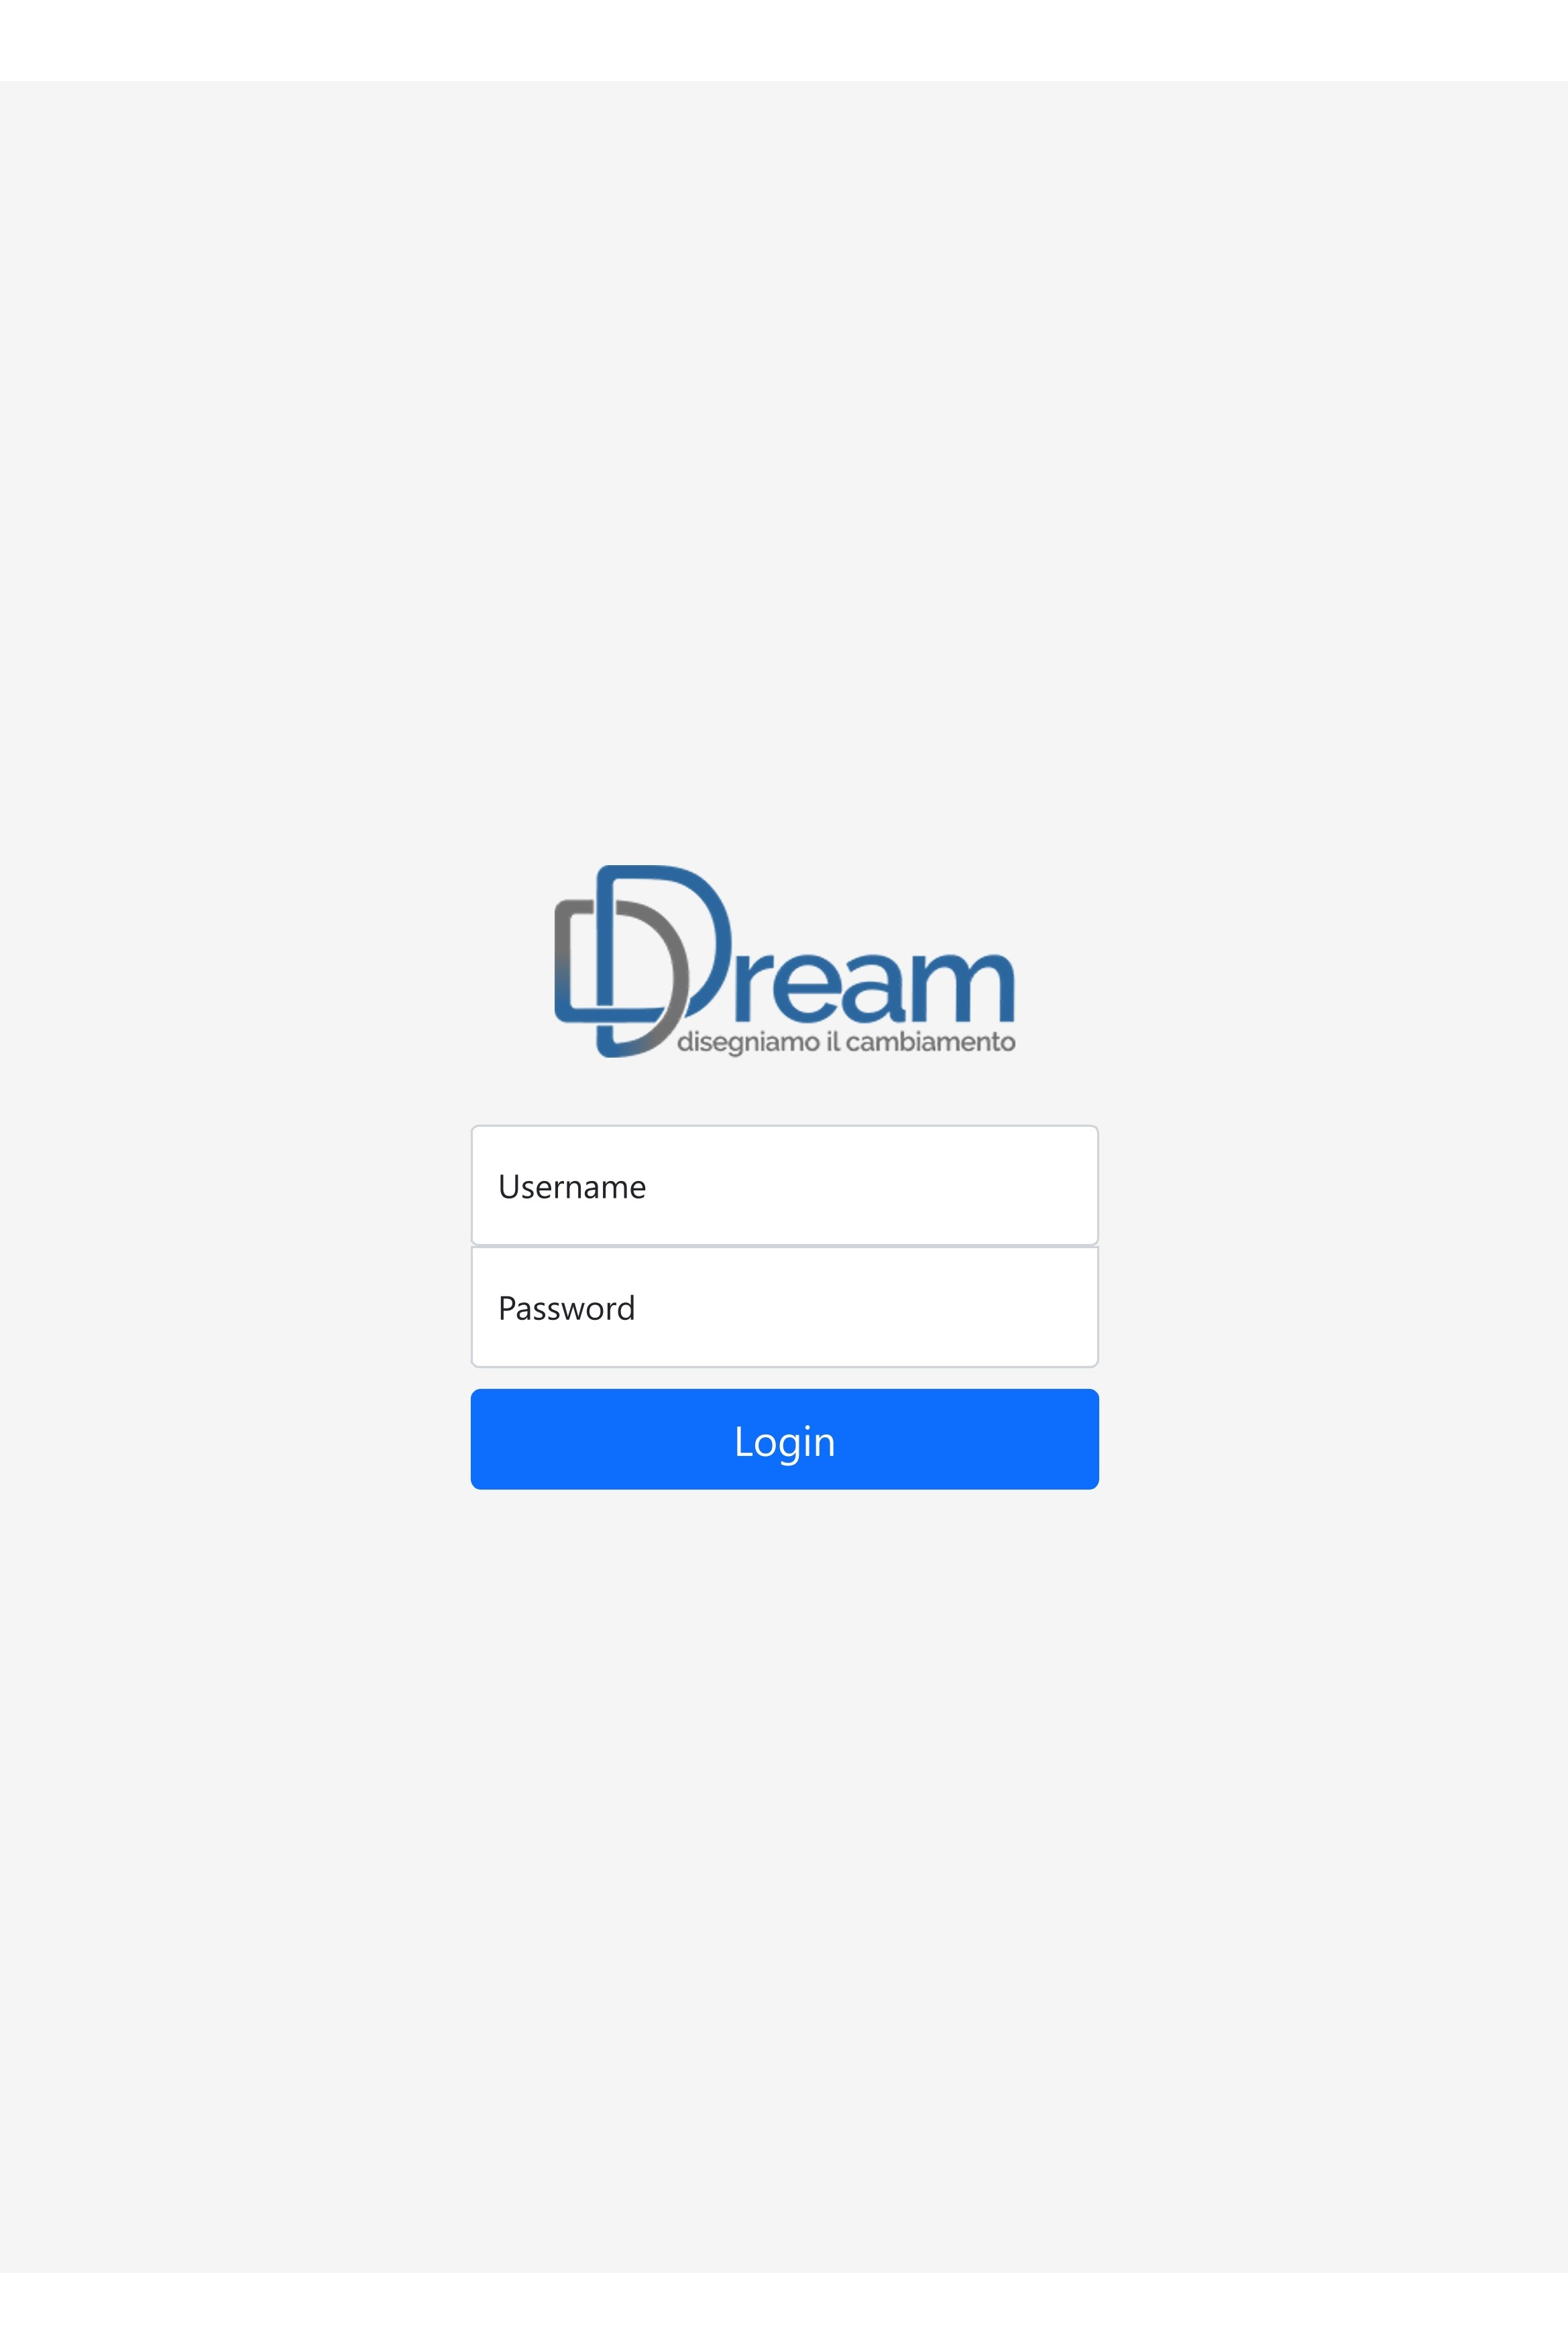
\includegraphics[width=\textwidth]{img/screen/Login-1.jpg}}
    \caption{Login (screenshot)}
    \label{fig:login}
  \end{minipage}
  \hfill
  \begin{minipage}[b]{0.65\textwidth}
    \fcolorbox{gray}{white}{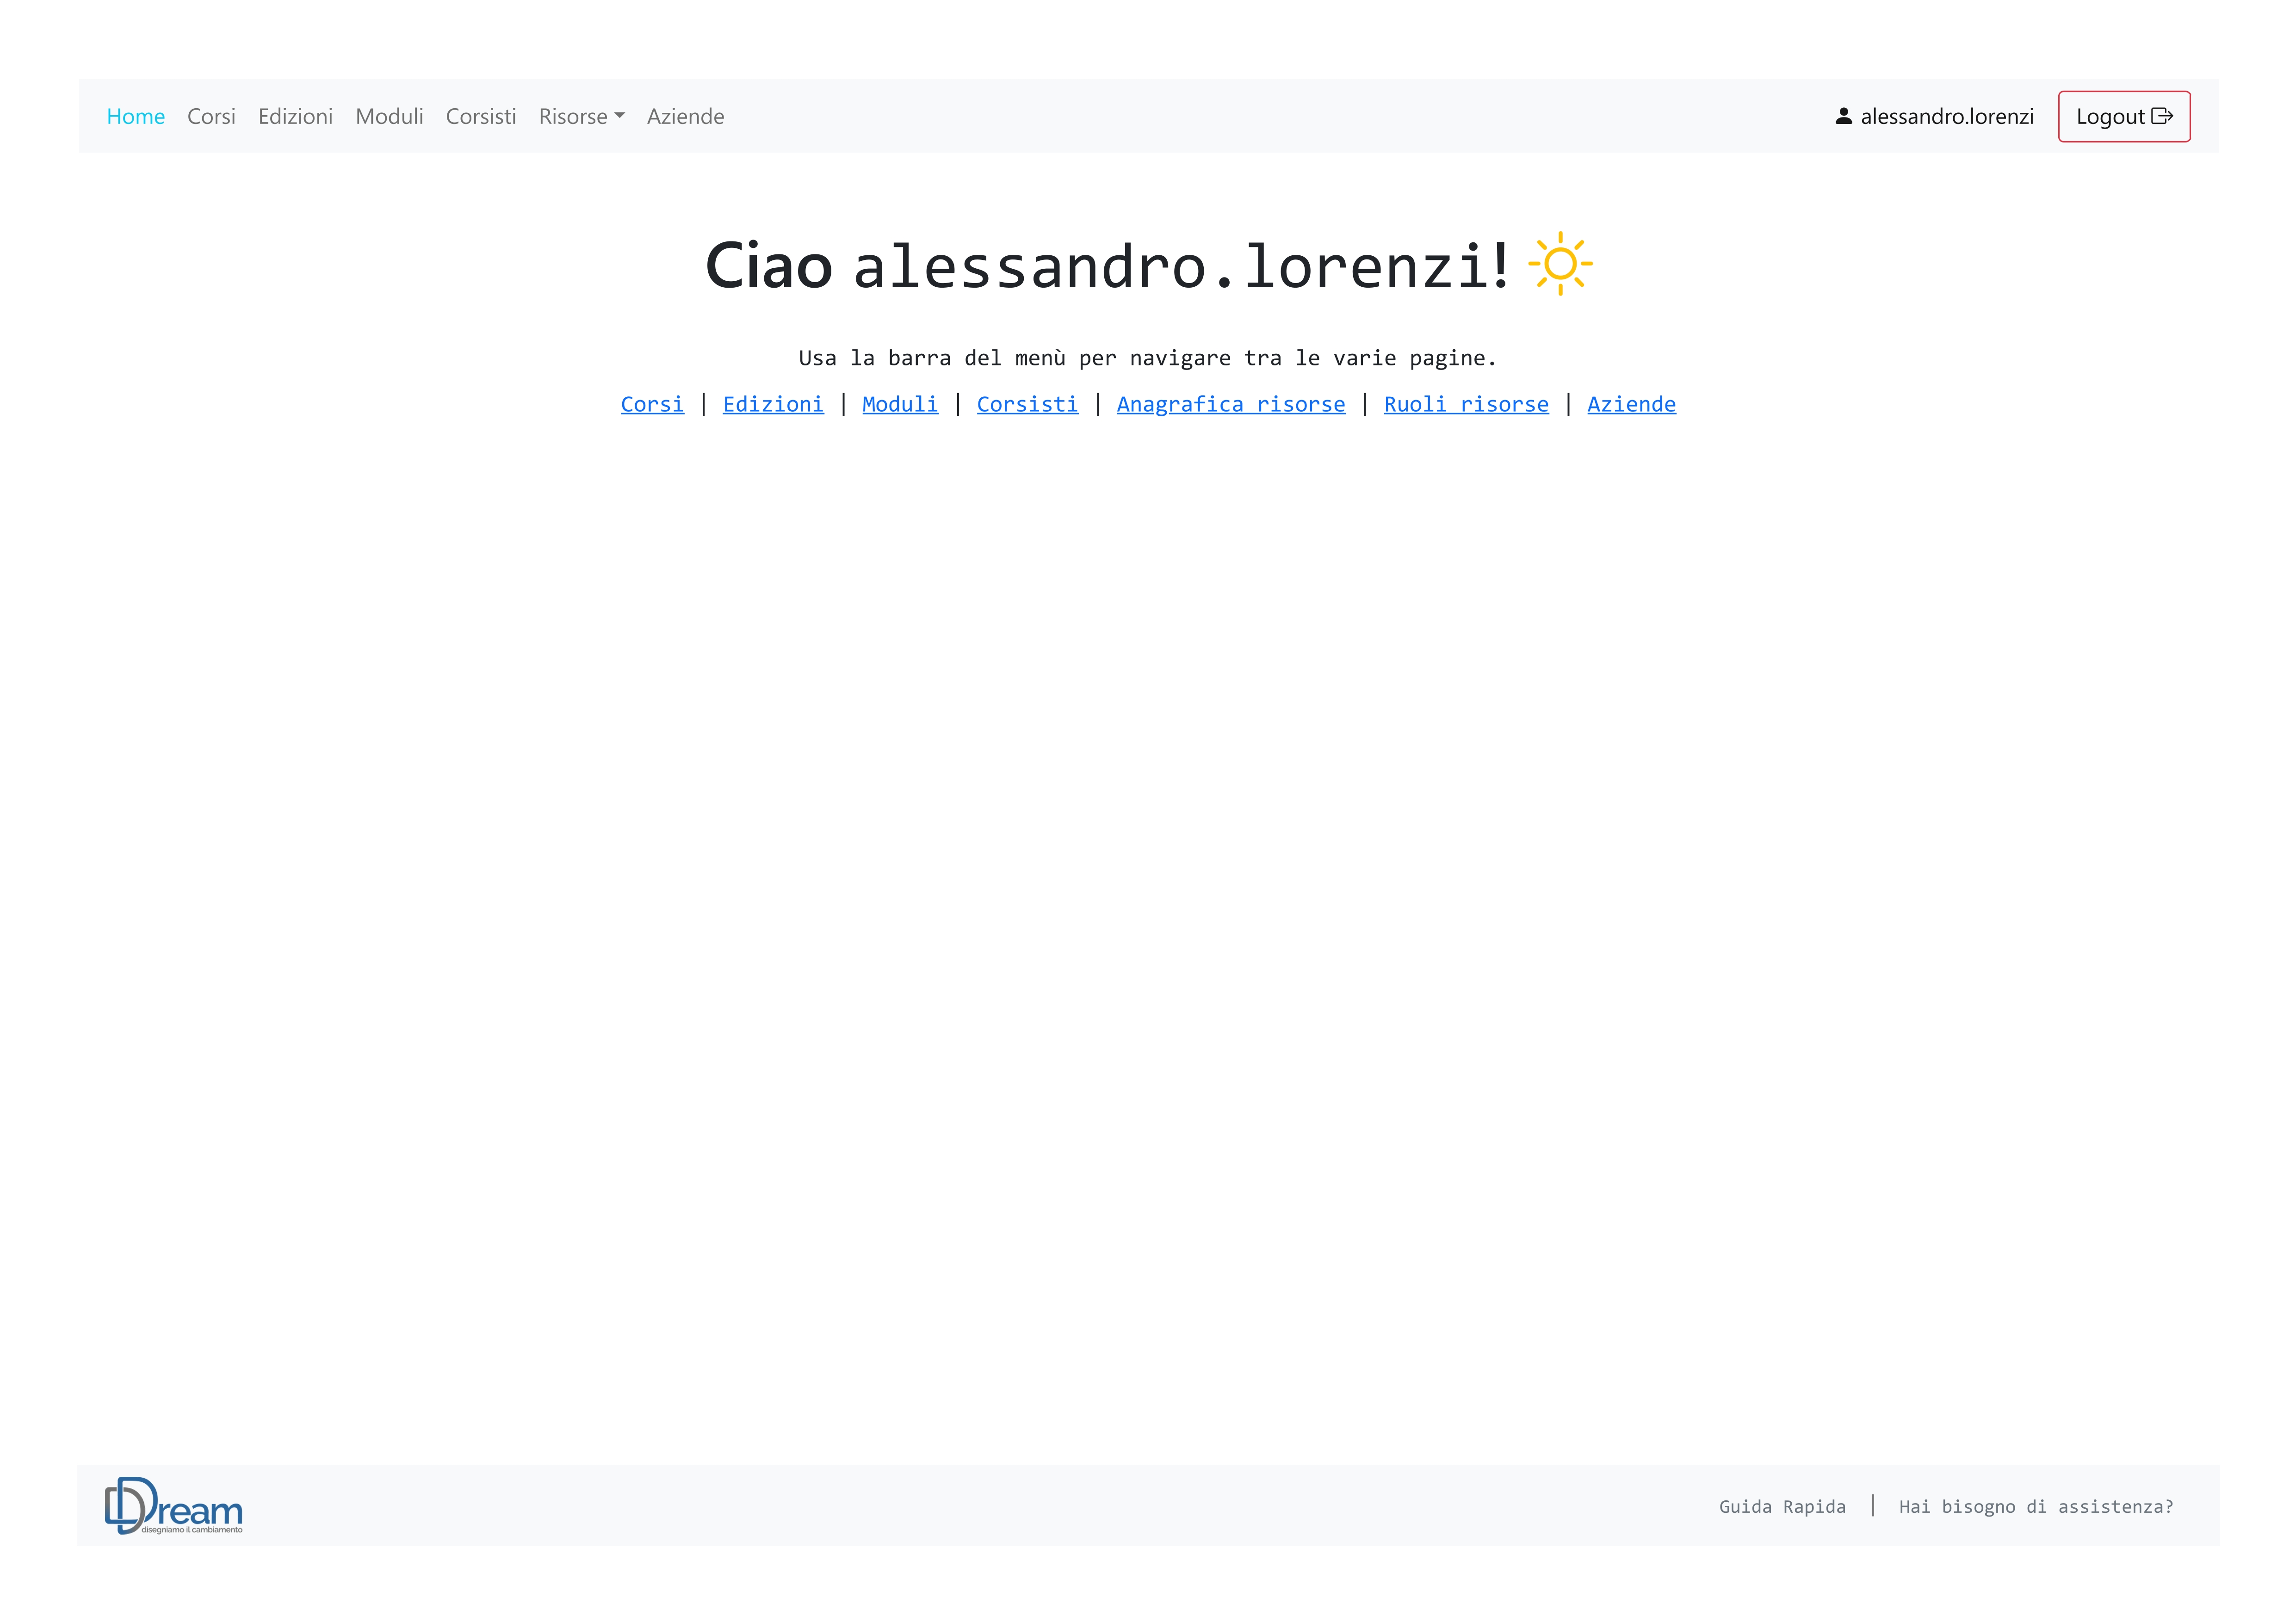
\includegraphics[width=\textwidth]{img/screen/Home-1.jpg}}
    \caption{Homepage (screenshot)}
    \label{fig:homepage}
  \end{minipage}
\end{figure}
\noindent
Le pagine \textit{Corsi}, \textit{Edizioni} e \textit{Moduli} permettono la gestione delle rispettive anagrafiche. L'utente può visualizzare in modo strutturato e navigabile le varie informazioni, aggiungere nuovi dati o eliminare i componenti presenti.

\section{Pagina Moduli}
La pagina \textit{Moduli} (figura \ref{fig:moduli}), un esempio tra le varie pagine di anagrafiche, fornisce una tabella che può essere filtrata per corso ed edizione. Ogni modulo può essere modificato e, se possibile, eliminato; l'utente può anche creare un nuovo modulo. 
\begin{figure}[!hbt]
\centering
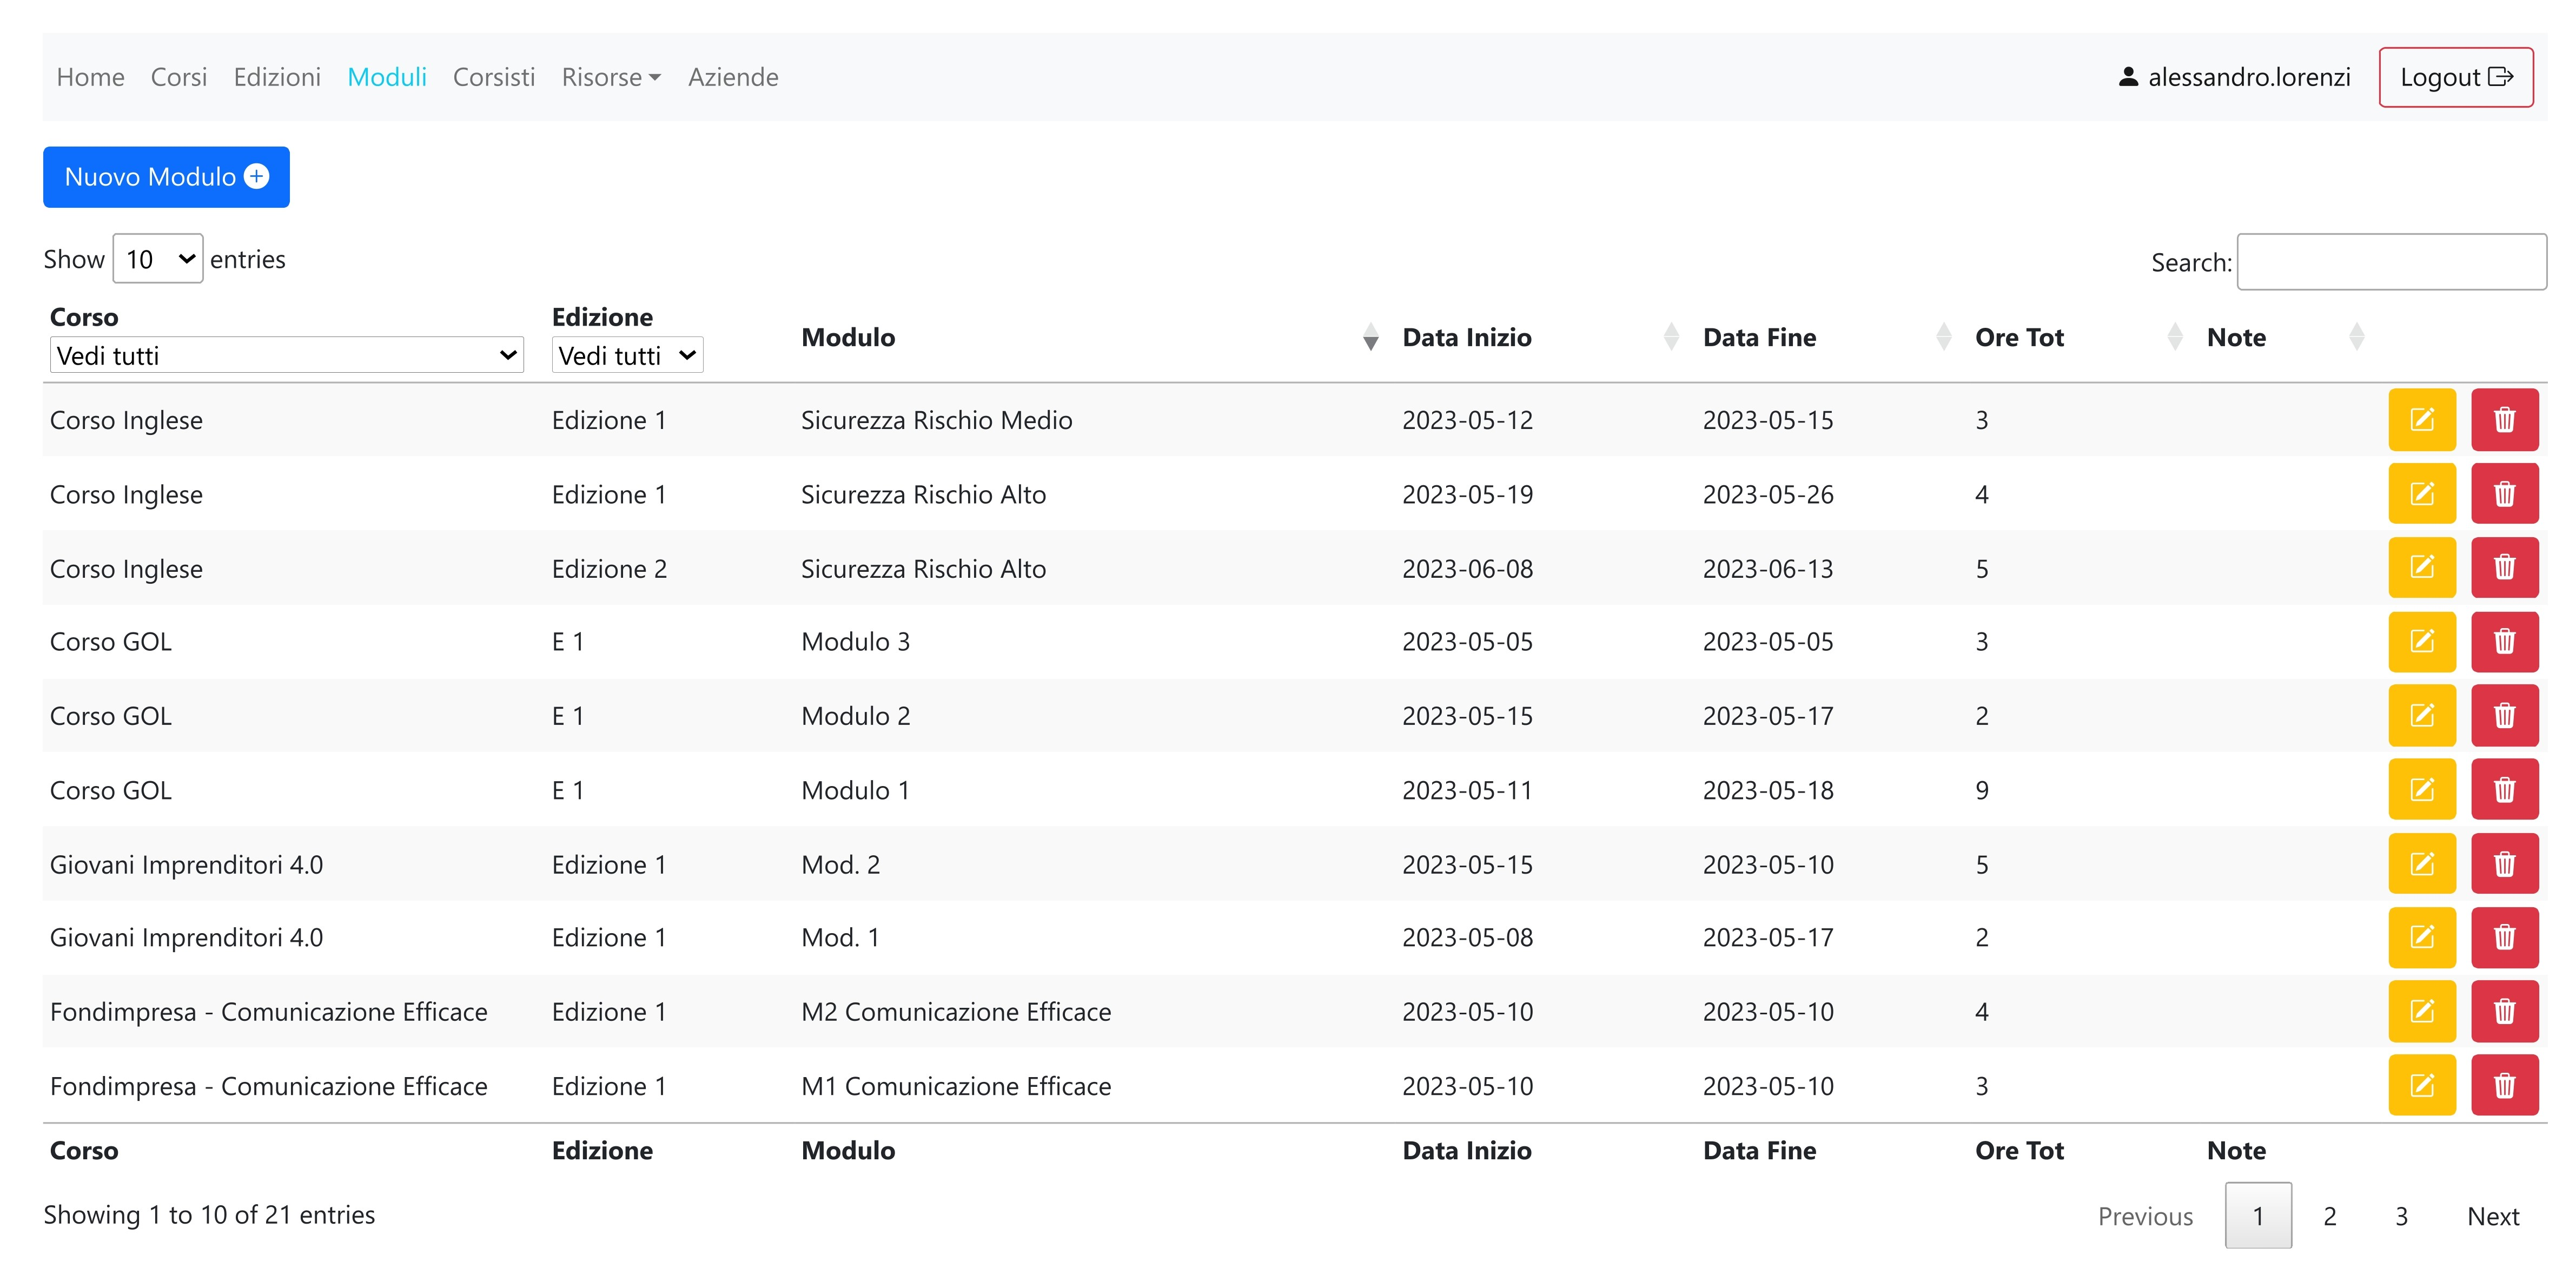
\includegraphics[scale=0.35]{img/screen/Moduli_tabella-1.jpg}
\caption{Pagina Moduli (screenshot)}
\label{fig:moduli}
\end{figure}
\newline
In figura \ref{fig:operazioni_moduli} si mostrano le operazioni di creazione e modifica di un modulo. In caso di creazione di un nuovo modulo il sistema popola due menù a discesa selezionabili che si aggiornano in base alle scelte fatte. Una volta compilati i campi obbligatori la nuova entità viene caricata nel database e la pagina di visualizzazione si aggiorna. In caso di modifica invece uno script in JavaScript precompila i campi del modulo selezionato e, una volta confermata la variazione, il sistema esegue l'aggiornamento delle informazioni aggiornando la tabella. Se l'utente dovesse scegliere di eliminare un elemento il gestionale controlla prima che non ci siano vincoli di integrità violati (ad esempio nel caso di moduli l'eliminazione è possibile solo se non ci sono corsisti e/o risorse associate a esso) e successivamente esegue la cancellazione o restituisce un messaggio di errore senza procedere.
\begin{figure}[!hbt]
\centering
% \begin{subfigure}{0.8\textwidth}
%      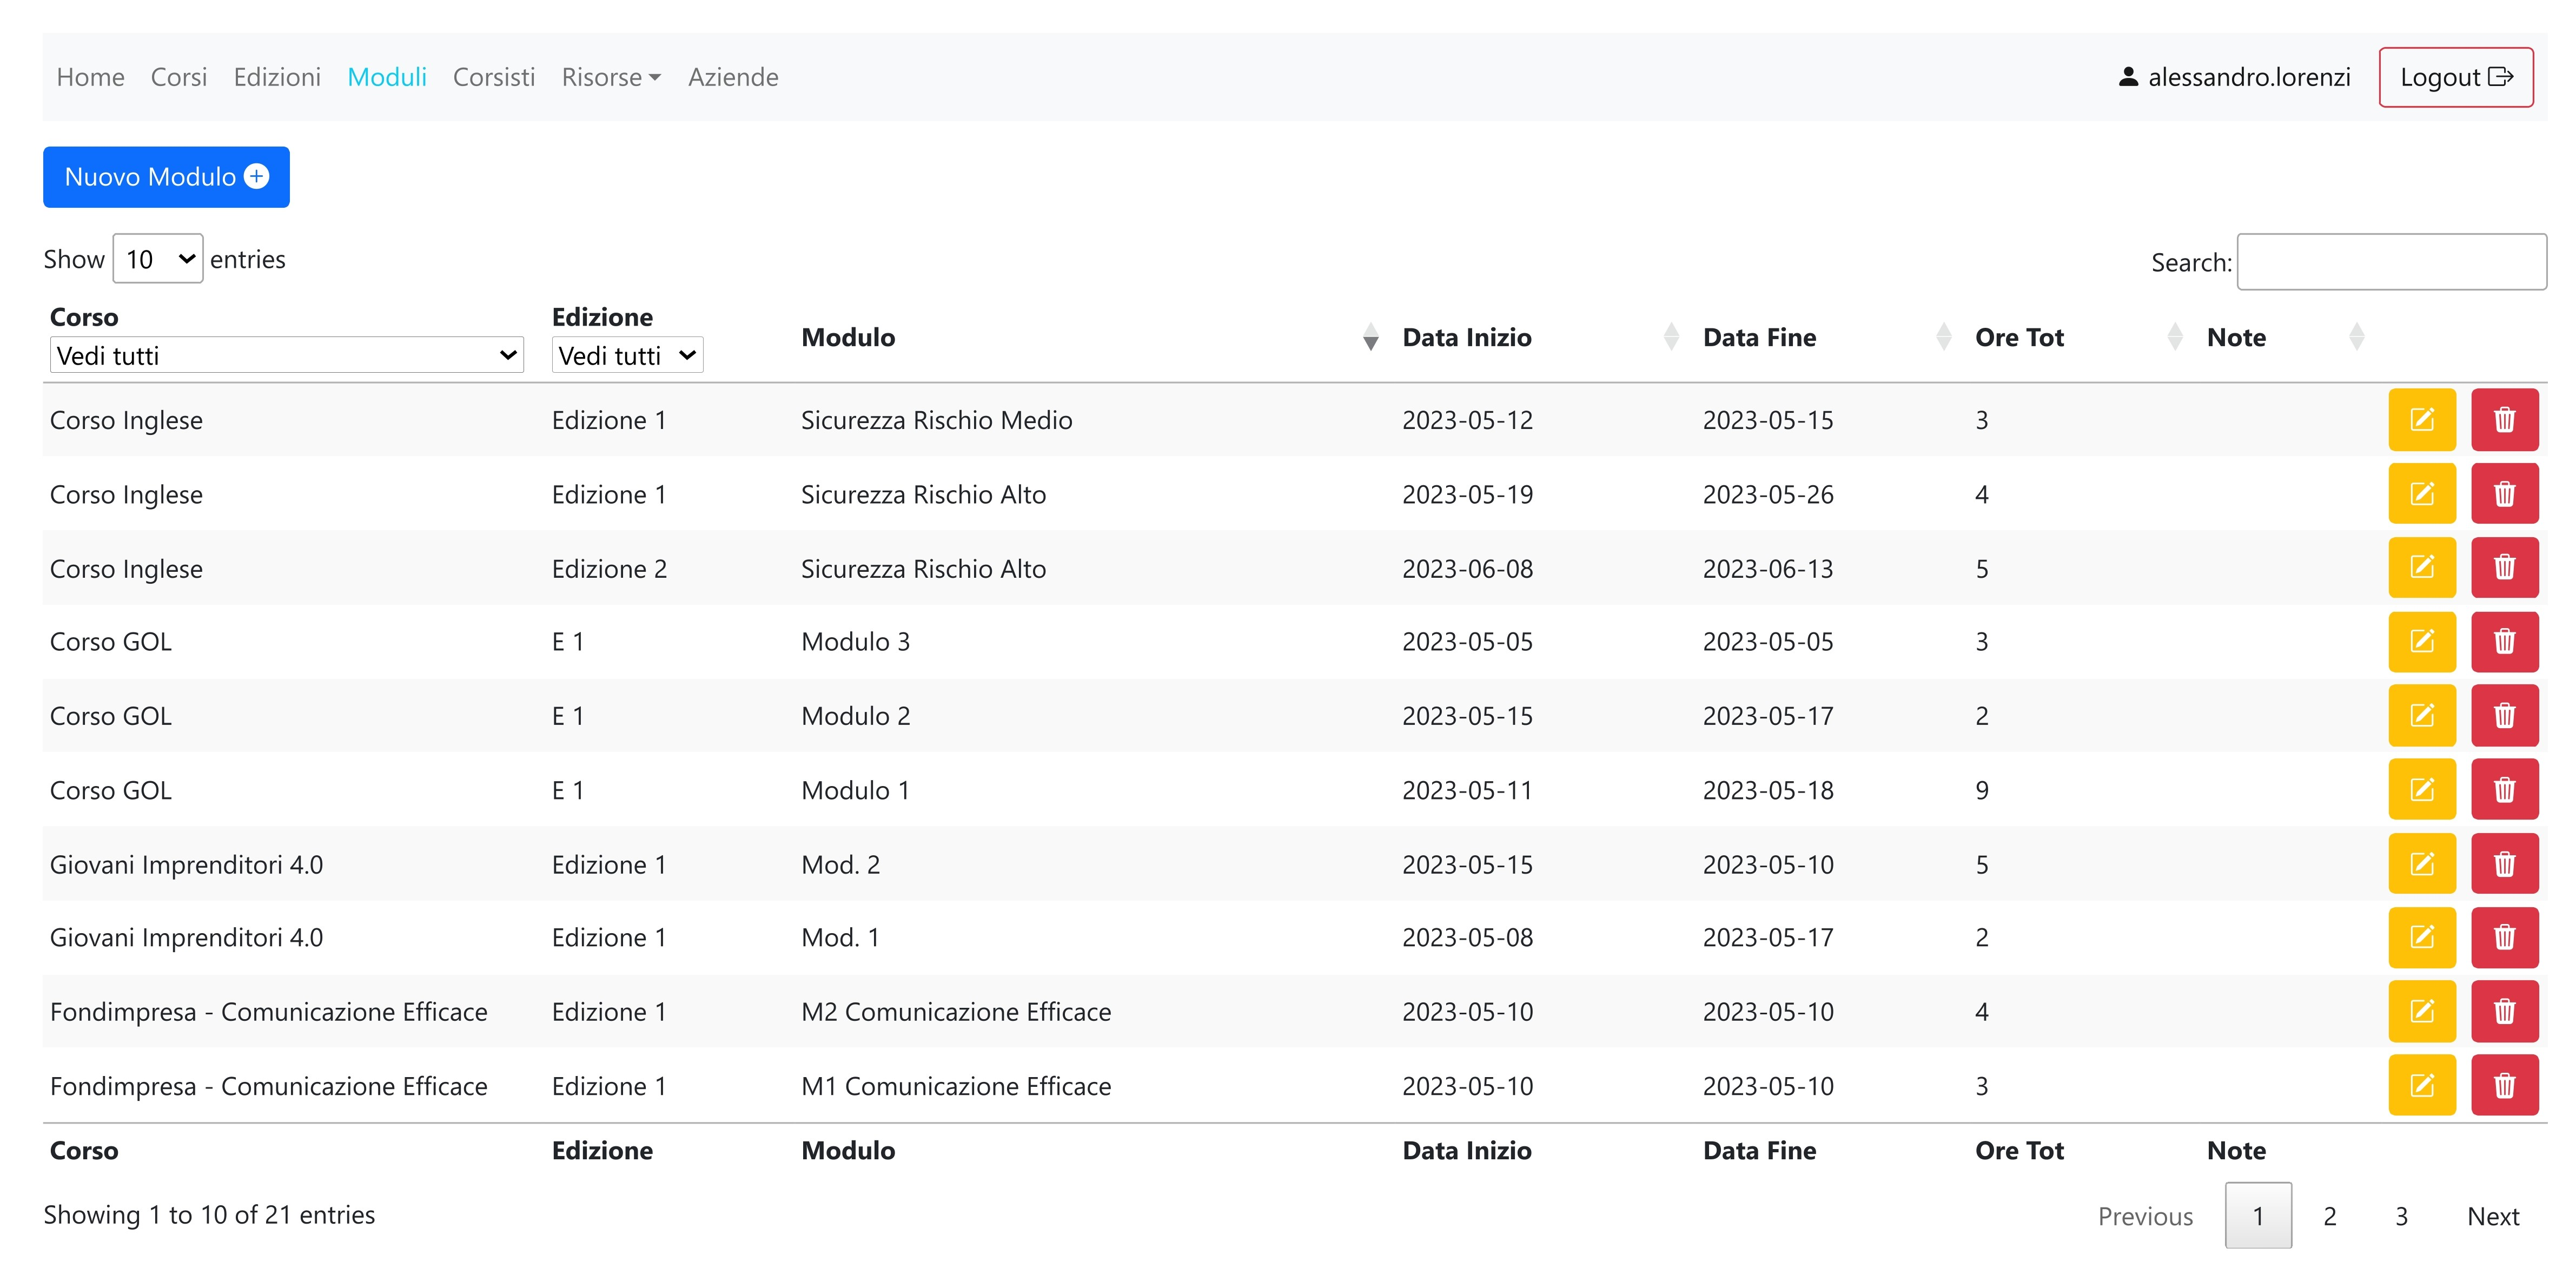
\includegraphics[width=\textwidth]{img/screen/Moduli_tabella-1.jpg}
%      \caption{Pagina Moduli}
%      \label{fig:nuovo_modulo}
%  \end{subfigure}
%  \hfill
 \begin{subfigure}{0.49\textwidth}
     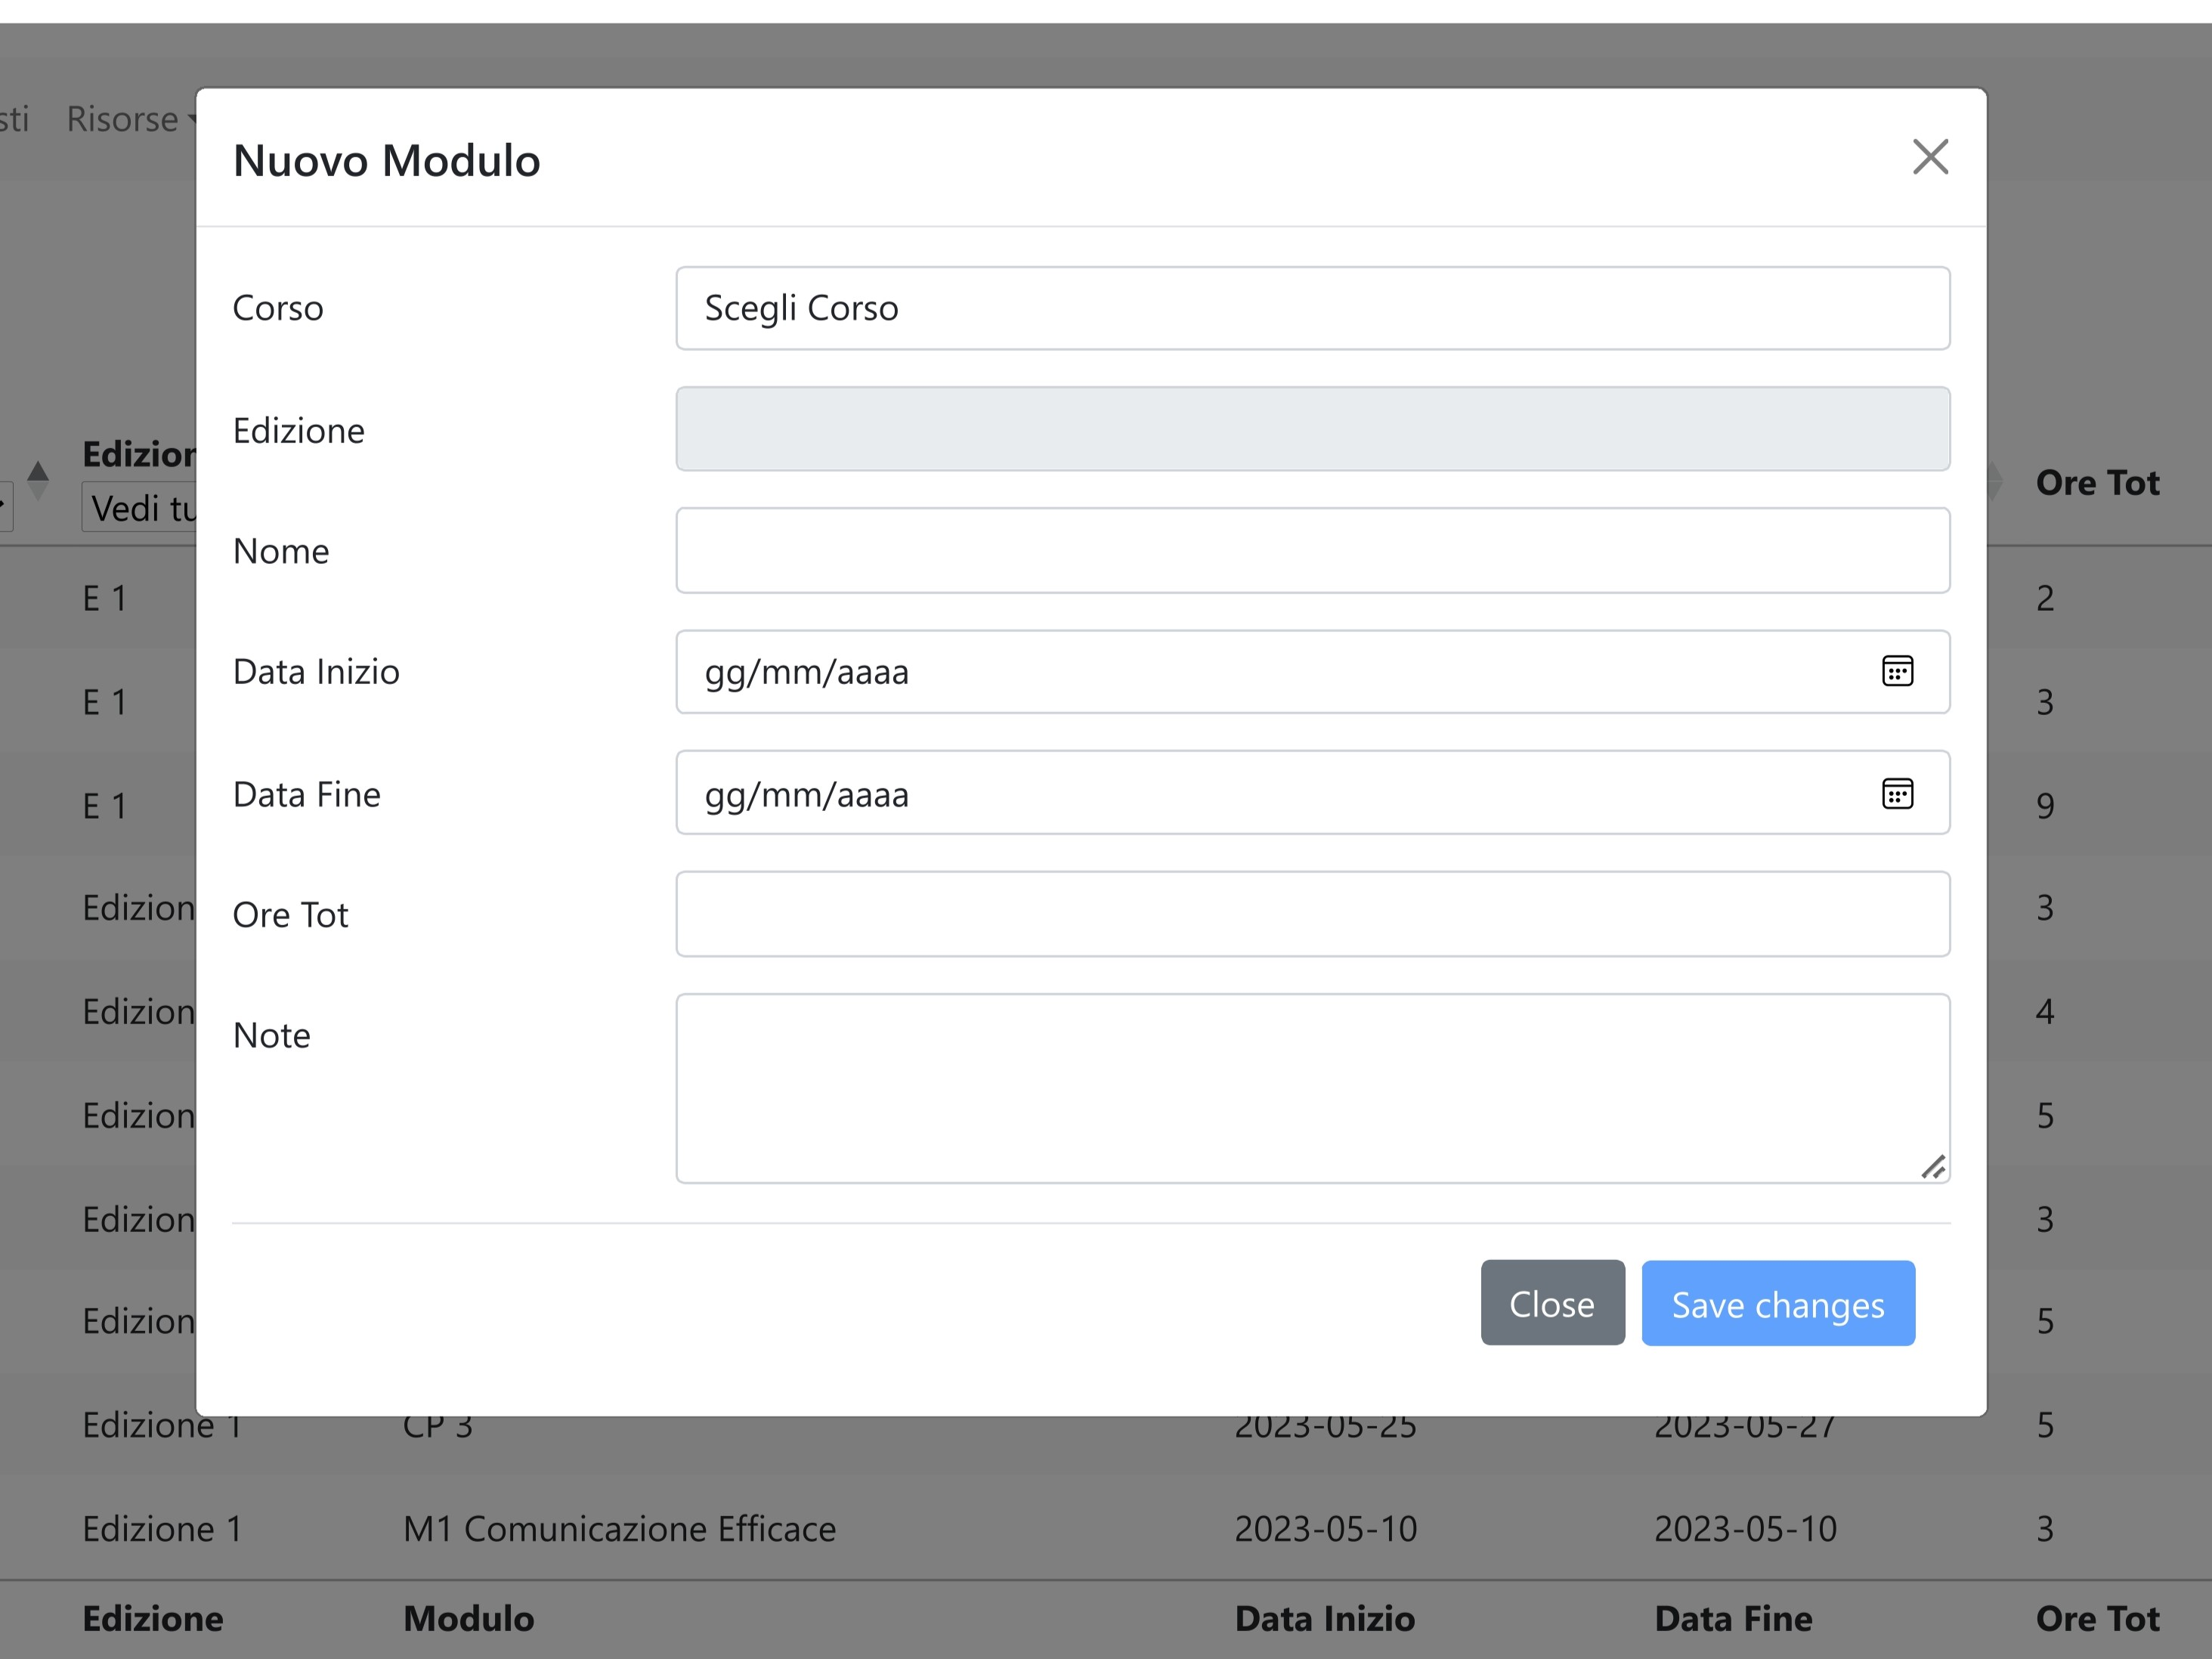
\includegraphics[width=\textwidth]{img/screen/Moduli_aggiungi-1.jpg}
     \caption{Nuovo Modulo}
     \label{fig:nuovo_modulo}
 \end{subfigure}
 \hfill
 \begin{subfigure}{0.49\textwidth}
     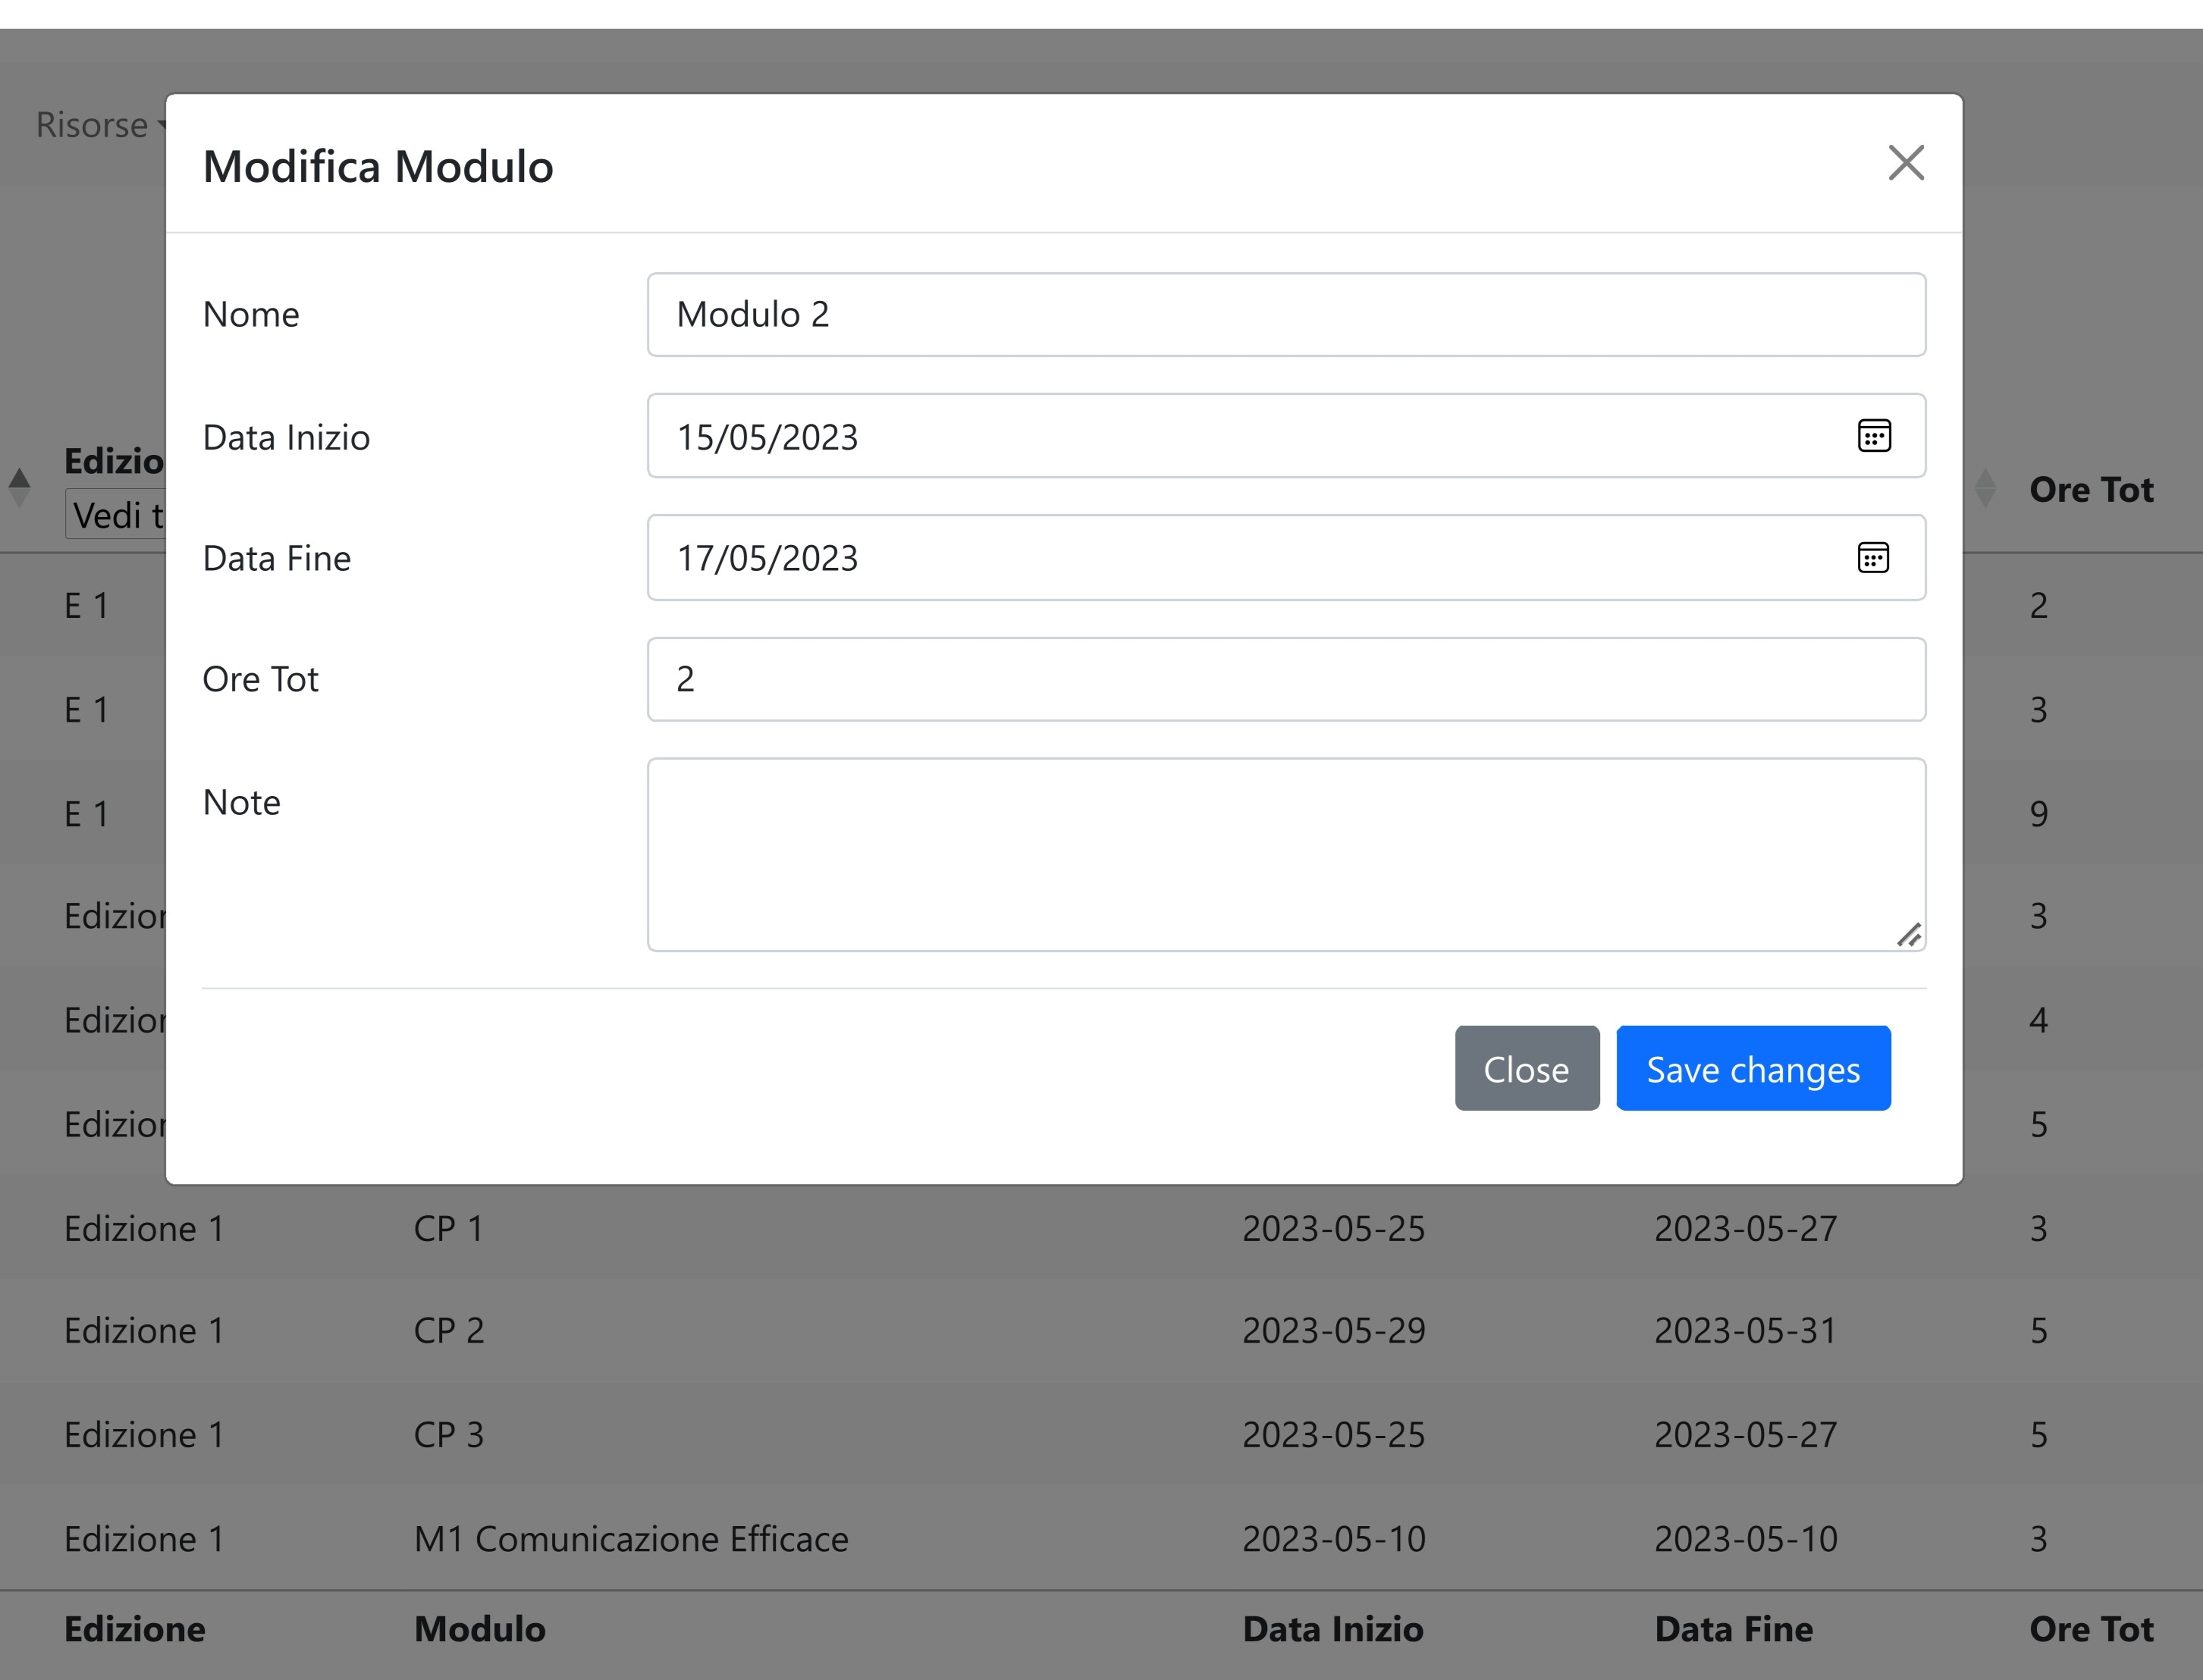
\includegraphics[width=\textwidth]{img/screen/Moduli_modifica-1.jpg}
     \caption{Modifica Modulo}
     \label{fig:modifica_modulo}
 \end{subfigure}
 %\hfill
% \begin{subfigure}{0.5\textwidth}
 %    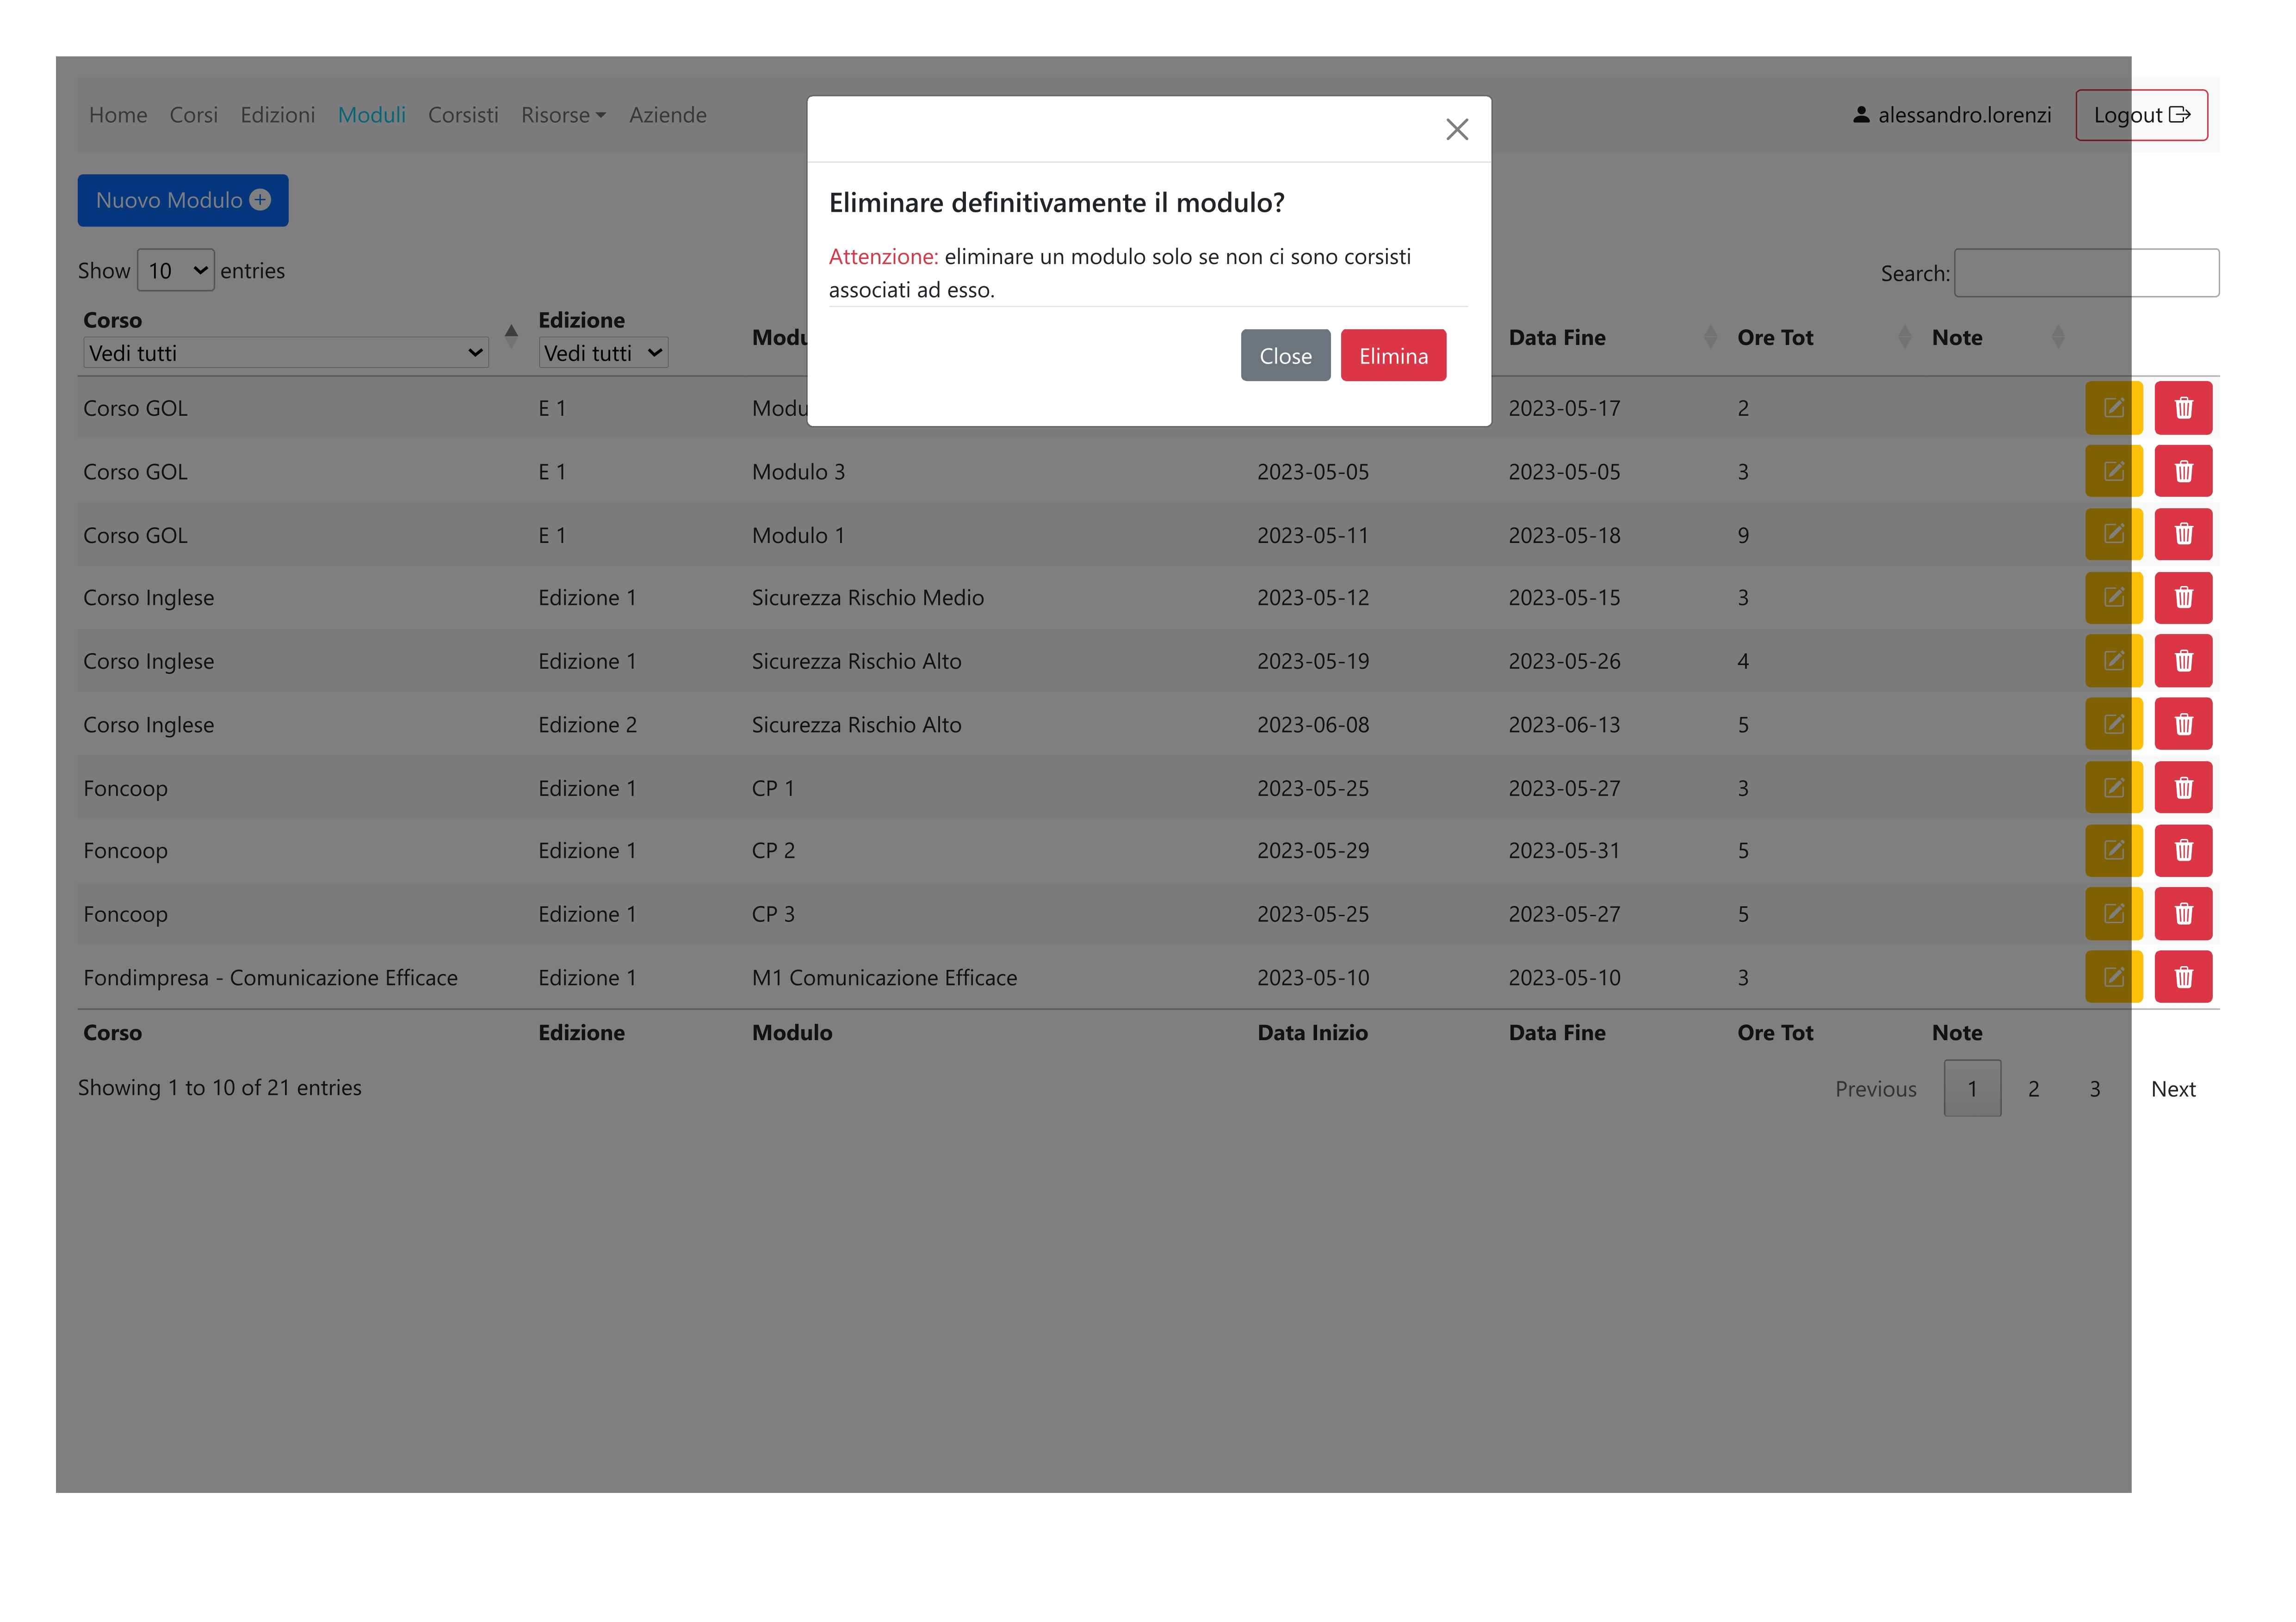
\includegraphics[width=\textwidth]{img/screen/Moduli_elimina-1.jpg}
  %   \caption{Elimina Modulo}
   %  \label{fig:elimina_modulo}
% \end{subfigure}
\caption{Operazioni sulla pagina Moduli}
\label{fig:operazioni_moduli}
\end{figure}
\newline
\section{Gestione Risorse}
Il gestionale fornisce due pagine per la gestione delle risorse e dei ruoli che queste hanno nei vari corsi: \textit{Anagrafica Risorse} e \textit{Ruoli Risorse}.
\subsection{Pagina Anagrafica Risorse}
Attraverso la pagina \textit{Anagrafica Risorse} (figura \ref{fig:risorse}) è possibile visualizzare in forma tabellare tutte le risorse, modificare o eliminare quelle già presenti o aggiungerne di nuove, nonché assegnare un ruolo a una figura specificando a quale modulo si riferisce e con che funzione. Questa sezione permette anche di vedere i documenti legati a ogni risorsa (come c.v., consensi della privacy o autorizzazioni varie). Per questa parte è stato inoltre implementato un sistema di notifiche che, al primo collegamento dell'utente, mostra quali documenti sono in scadenza (ogni tipo ha una sua scadenza).
\begin{figure}[!hbt]
\centering
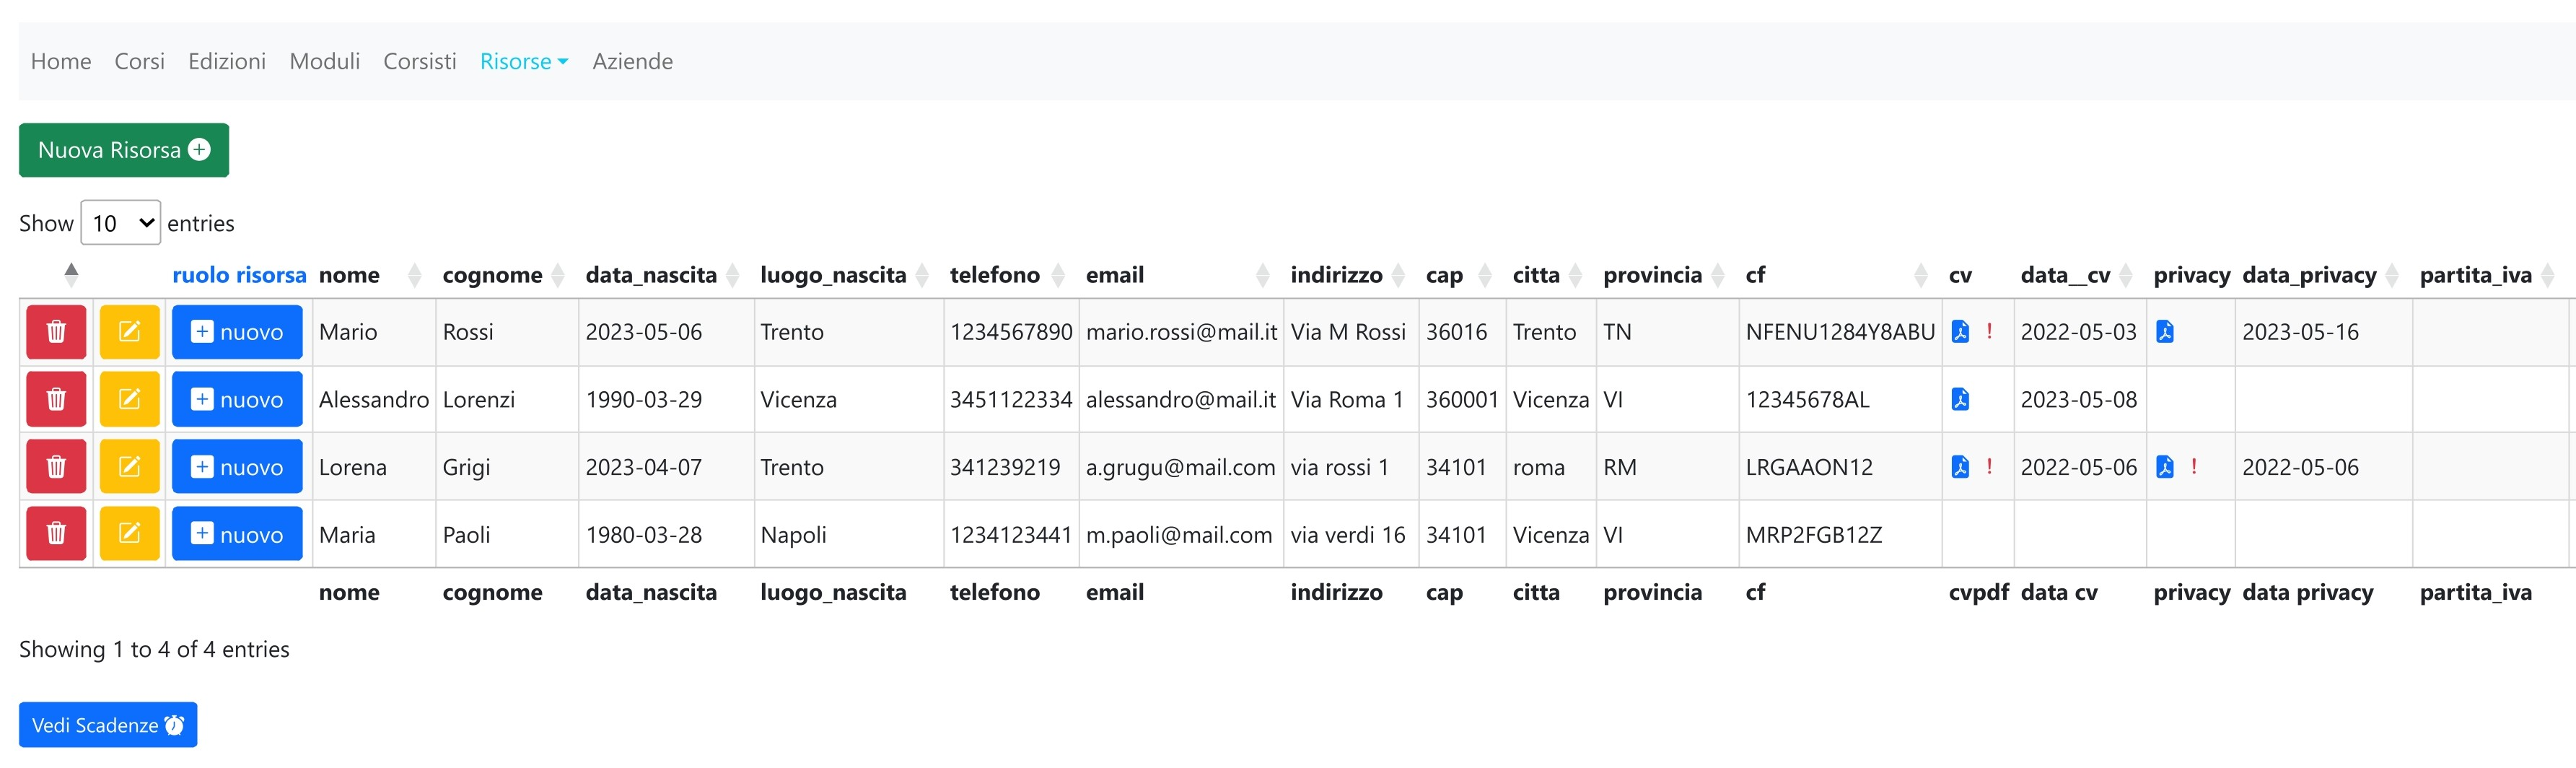
\includegraphics[scale=0.55]{img/screen/Risorse-1.jpg}
\caption{Pagina Anagrafica Risorse (screenshot)}
\label{fig:risorse}
\end{figure}
\newline
\newline
La gestione dei file PDF in un gestionale è sempre una questione delicata da trattare. In questo caso si è scelto di creare delle tabelle apposite per la memorizzazione nel database (come illustrato nello schema EER in figura \ref{fig:DiagrammaEER}), ognuna delle quali ha una struttura simile e utilizza il formato \textit{BLOB} (Binary large object) \cite{blob} per l'archiviazione di file di medie o grandi dimensioni, allocando quindi lo spazio necessario solo quando viene effettivamente utilizzato il contenuto del campo.\newline
Nel frammento di codice adattato (listing  \ref{code:blob}) si mostra come è stato gestito il caricamento di un file PDF con relativa query nel database; la parte di codice successiva (listing \ref{code:get_cv}) serve invece a restituire e mostrare il file richiesto della risorsa selezionata in modo corretto.
\begin{listing}[!hbt]
\begin{minted}{PHP}
<?php 
...
if ($_FILES['cv-risorsa']['size'] > 0) {
    $fileName = $_FILES['cv-risorsa']['name'];
    $tmpName  = $_FILES['cv-risorsa']['tmp_name'];
    $fileSize = $_FILES['cv-risorsa']['size'];
    $fileType = $_FILES['cv-risorsa']['type'];

    $fp = fopen($tmpName, 'r');
    $content = fread($fp, filesize($tmpName));
    $content = addslashes($content);
    fclose($fp);

    $fileName = addslashes($fileName);

    $query .= "SET @CVid = (SELECT LAST_INSERT_ID(pdf_cv.id_cv) from pdf_cv
    order by LAST_INSERT_ID(pdf_cv.id_cv) desc limit 1) + 1;"; //get id_cv_pdf
    $query .= "INSERT INTO pdf_cv (id_cv, filename,file_cv) " .
        "VALUES (@CVid, '$fileName', '$content');"; //insert pdf cv
    $query .= "SET @CVdate =  CURRENT_DATE;"; //set date cv
} else {
    $query .= "SET @CVid = null; SET @CVdate = null;";
}
...
\end{minted}
\caption{inserimento file BLOB in database}
\label{code:blob}
\end{listing}
\begin{listing}[!hbt]
\begin{minted}{PHP}
<?php
if (isset($_GET["id"])) {
    ...
    $id = $_GET["id"];
    if ($id != "null") {
        $query = "SELECT filename, file_cv FROM pdf_cv WHERE id_cv = '$id'";
        $result = $conn->query($query) or die($conn->error);
        $row = mysqli_fetch_assoc($result);

        header("Content-type: application/pdf");
        header('Content-disposition: inline; filename=' . $row["filename"] .
        '.pdf');
        header('Content-Transfer-Encoding: binary');
        header('Accept-Ranges: bytes');
        
        echo $row["file_cv"];
    } else {
        echo "<div>file non disponibile</div><a href='' 
        onclick='window.close()'>torna indietro</a>";
    }
    ...
}
\end{minted}
\caption{Interrogazione al database per ottenere e mostrare un file}
\label{code:get_cv}
\end{listing}

\subsection{Pagina Ruoli Risorse}
La pagina \textit{Ruoli Risorse} (figura \ref{fig:ruoli}) permette di visualizzare, filtrare e gestire le figure impegnate in uno o più moduli dei corsi presenti. Ogni risorsa può avere un ruolo diverso (docente, tutor, coordinatore, ecc.) nello stesso modulo ed essere assegnato a più moduli e corsi. Se quindi attraverso la pagina \textit{Anagrafica Risorse} è possibile effettuare l'assegnazione \textit{Risorsa-Ruolo} specificandone le informazioni necessarie, in questa pagina avviene l'amministrazione di esse.
\begin{figure}[!hbt]
\centering
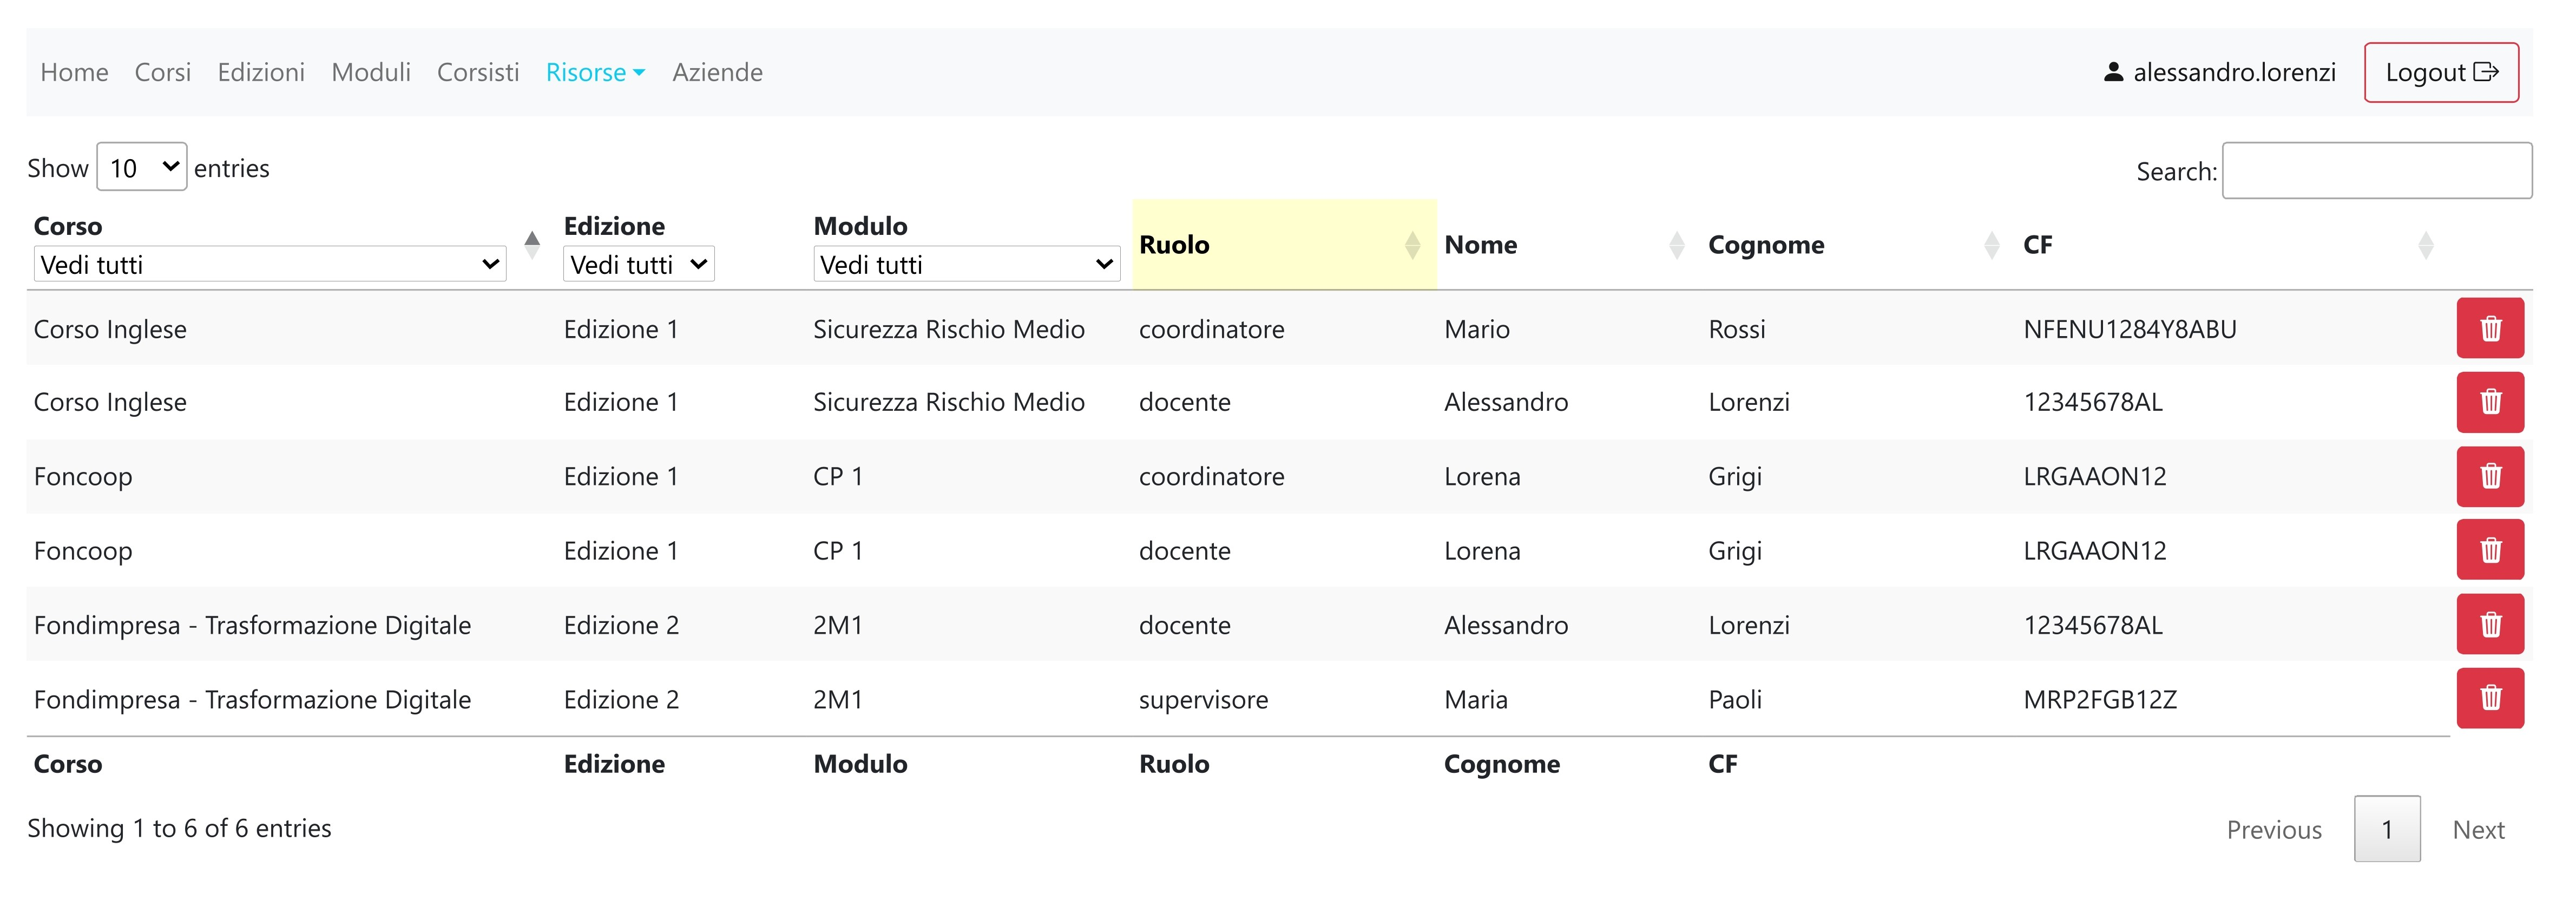
\includegraphics[scale=0.40]{img/screen/Ruoli-1.jpg}
\caption{Pagina Ruoli Risorse (screenshot)}
\label{fig:ruoli}
\end{figure}
\newline
\section{Pagina Corsisti}
La pagina \textit{Corsisti} (figura \ref{fig:corsisti}) include tutte le funzioni necessarie per la gestione di questa anagrafica. Oltre alle operazioni precedentemente descritte per le altre pagine, da quest'area l'utente può:
\begin{itemize}
  \item Scaricare gli attestati personalizzati di tutti i corsisti di un'edizione di un corso (sezione \ref{sec:attestati}).
  \item Caricare massivamente i corsisti tramite vari modelli Excel prestabiliti. Il sistema inserire quindi i dati delle nuove figure e associa ad esse tutti i moduli presenti in quell'edizione (sezione \ref{sec:excel}).
\end{itemize}
\noindent
\begin{figure}[!h]
\centering
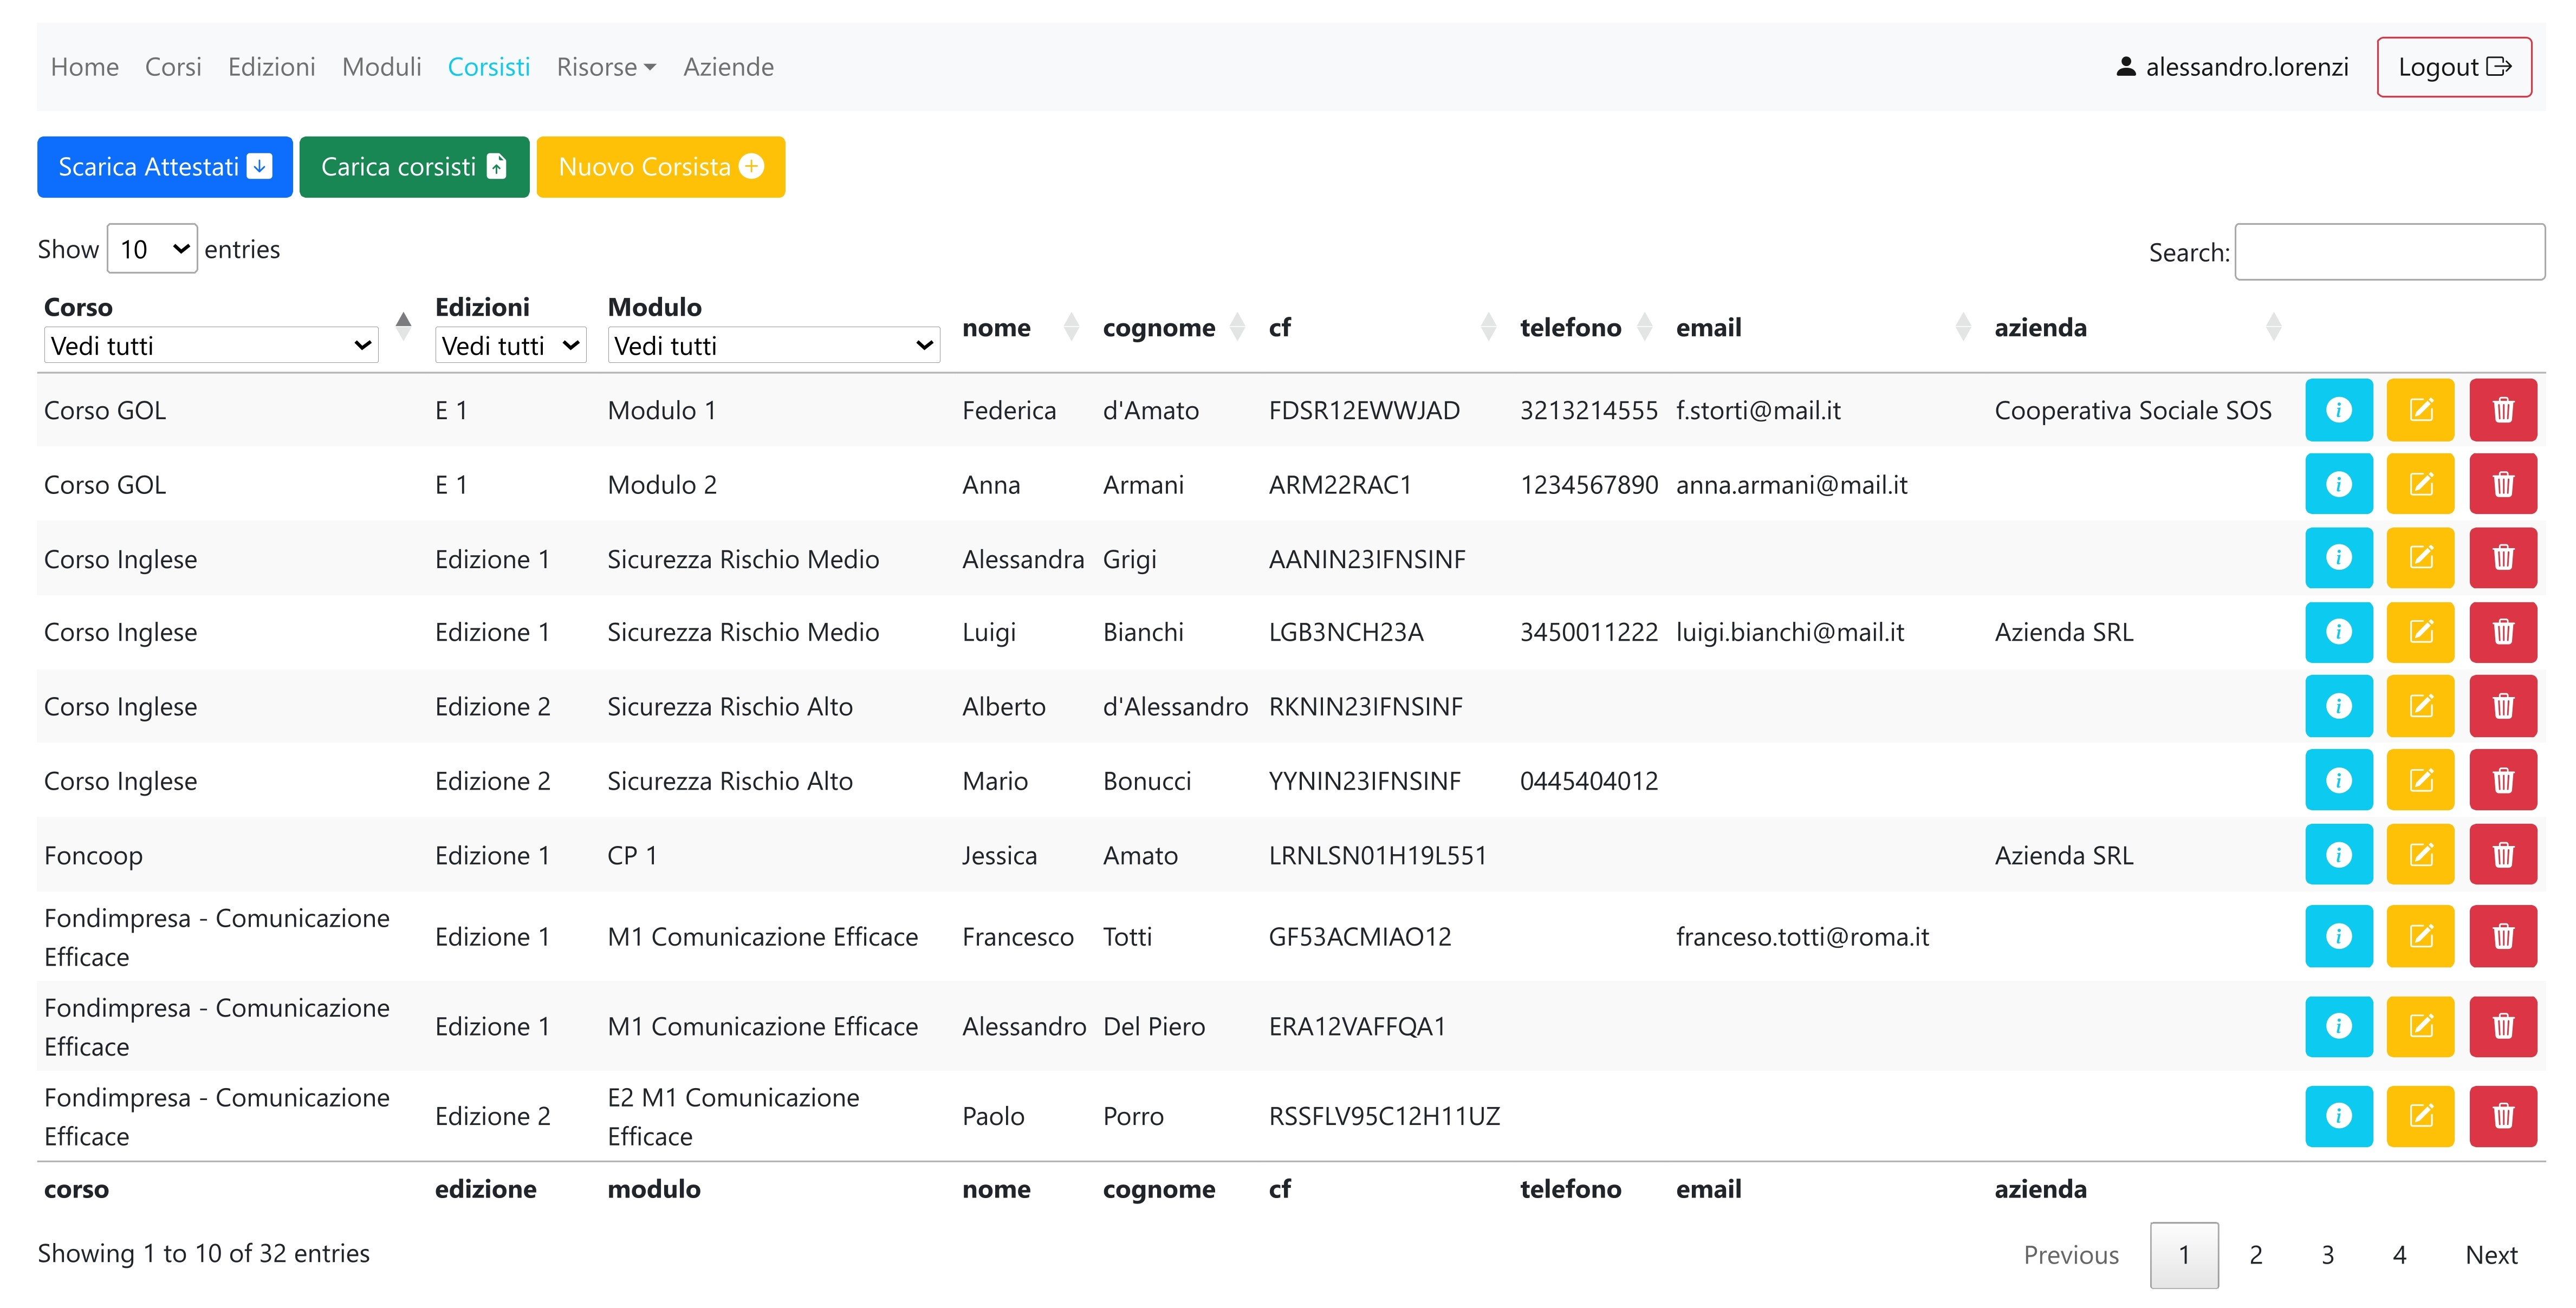
\includegraphics[scale=0.40]{img/screen/Corsisti-1.jpg}
\caption{Pagina Corsisti (screenshot)}
\label{fig:corsisti}
\end{figure}
\noindent
\subsection{Generazione di documenti}
\label{sec:attestati}
La funzione di generazione degli attestati è stata implementata usando FPDF \cite{fpdf}, classe PHP che in maniera semplice e con funzioni ad alto livello permette di generare PDF senza l'uso di altre librerie esterne più complesse e creando modelli predefiniti che vengono elaborati con dati specifici. Di seguito si riporta una frammento di codice adattato (listing \ref{code:fpdf185}) usato per generare un modello di attestato personalizzato per ogni corsista e per creare la cartella \verb|.zip| da scaricare. Il primo blocco di codice crea e riempie la cartella mentre il secondo elabora il file PDF. 
\begin{listing}[!hbt]
\begin{minted}{PHP}
<?php 
...
if ($result->num_rows > 0) {
    $zip = new ZipArchive();
    $zip->open('./test.zip', ZIPARCHIVE::OVERWRITE | ZIPARCHIVE::CREATE);
    while ($row = $result->fetch_assoc()) {
        $file = creaAttestato(... data ...);
        $zip->addFile($file);
    }
    $zip->close();
    
    $folder_path = "./";
    $files = glob($folder_path . '/*.pdf');
    foreach ($files as $file) {
        if (is_file($file)) {
            unlink($file);
        }
    }
    ...
}

...
function creaAttestato(... data ...)
{
    $pdf = new FPDF('P', 'mm', 'A4');
    $pdf->AddPage();
    $pdf->SetFont('Arial', 'I', 7);

    //write pdf ...
    
    $file = trim($nome) . '_' . trim($cognome) . '.pdf';
    trim($nome) . '_' . trim($cognome) . '.pdf';
    $pdf->Output($file, 'F');
    return $file;
}
\end{minted}
\caption{fpdf185 in PHP}
\label{code:fpdf185}
\end{listing}
\noindent
\newline

\subsection{Gestione di fogli elettronici}
\label{sec:excel}
Per la lettura dei dati dai fogli elettronici è stata scelta la classe SimpleXLSX \cite{simpleXLSX} che, senza estensioni aggiuntive, analizza, recupera ed effettua il parsing dei dati dai file Excel. Lo script di codice adattato riportato (listing \ref{code:simpleXLSX}) mostra la lettura dei dati da file \verb|.xlsx| a cui poi seguirà l'importazione a database.
\begin{listing}[!hbt]
\begin{minted}{PHP}

<?php 
...
use Shuchkin\SimpleXLSX;
ini_set('error_reporting', E_ALL);
ini_set('display_errors', true);
if ($xlsx = SimpleXLSX::parse($_FILES['file']['tmp_name'])){
    ...
    $dim = $xlsx->dimension();
    $cols = $dim[0];
    foreach ($xlsx->readRows() as $k => $r) {
        if ($k < 4) continue; // skip firsts 4 rows

            if ($r[10] != "") { //stop
                if ($r[18] != '') //check if "azienda" is NULL
                    $query = "INSERT INTO corsista (id_corsista, nome, cognome,
                    data_nascita, luogo_nascita, sesso, cf, telefono, email,
                    indirizzo, cap, citta, provincia, cittadinanza, titolo_studio,
                    categoria, intestatario_cc, coordinate_cc, tipo_contratto,
                    data_assunzione, note, azienda_cf, inquadramento) VALUES 
                    (NULL,'$r[1]', '$r[0]', '$r[2]', '$r[6]', '$r[3]', '$r[10]',NULL,
                    NULL, NULL, NULL, NULL, NULL, '$r[7]', '$r[11]', NULL, NULL, NULL,
                    '$r[12]', '$r[16]', NULL, '$r[18]', '$r[15]');";


                //get id_corsista
                $query .= "SET @CorsistaID = (SELECT LAST_INSERT_ID(
                corsista.id_corsista) from corsista order by LAST_INSERT_ID(
                corsista.id_corsista) desc limit 1);";

                //insert corso - edizione
                $query .= "INSERT INTO corsista_modulo SELECT NULL, @CorsistaID,
                m.id_modulo, 1 FROM modulo m INNER JOIN edizione e on m.edizione
                = e.id_edizione INNER JOIN corso co on e.corso = co.id_corso 
                WHERE co.id_corso = '$corso' AND e.id_edizione = '$edizione'";

                //run multi_query
                $conn->multi_query($query);
                while (mysqli_more_results($conn)) {
                    mysqli_next_result($conn);
                }
                if ($conn->multi_query($query) == FALSE) {
                    echo "Error: " . $query . "<br>" . $conn->error;
                }
            }
        }
    }
} else {
    echo SimpleXLSX::parseError();
}
\end{minted}
\caption{SimpleXLSX in PHP}
\label{code:simpleXLSX}
\end{listing}
\section{Pagina Pubblica}
Un'altra richiesta implementata è stata quella di avere una pagina pubblica raggiungibile da possibili docenti esterni che, completando un modulo di registrazione, vengono inseriti a sistema e quindi mostrati nella pagina delle risorse per poi potenzialmente essere associati a un ruolo. In figura \ref{fig:public} si mostra la pagina pubblica menzionata. Questo modulo è l'unico che non richiede l'accesso con credenziali. Il gestionale effettua una serie di controlli di correttezza dei dati compilati prima di procedere con l'effettiva memorizzazione nel database. 
\begin{figure}[!hbt]
\centering

\includegraphics[scale=0.50]{img/screen/Public.jpg}
\caption{Pagina pubblica per risorse (screenshot)}
\label{fig:public}
\end{figure}
\clearpage
\newpage

